\documentclass[UTF8,a4paper,zihao=5,fontset=none]{ctexart}
\usepackage[margin=23mm,headheight=15pt,headsep=7mm]{geometry}
\usepackage{fontspec}
\setmainfont{TeX Gyre Termes}
\setsansfont{TeX Gyre Heros}
\setmonofont{DejaVu Sans Mono}[Scale=.82]
\setCJKmainfont{Source Han Serif SC}[ItalicFont={Source Han Serif SC},ItalicFeatures={FakeSlant=.15}]
\setCJKsansfont{Noto Sans SC}[AutoFakeBold=2]
\setCJKmonofont{Noto Sans SC}
\usepackage{amsmath,amssymb,mathtools,booktabs,longtable,tabularx,array}
\usepackage{graphicx,enumitem,xcolor,tikz,fancyhdr,listings,caption,microtype}
\usepackage[section]{placeins}
\usepackage{needspace}
\usepackage[most]{tcolorbox}
\usepackage[numbers,sort&compress]{natbib}
\usepackage{xurl}
\usepackage[colorlinks=true,linkcolor=blue!45!black,citecolor=blue!45!black,urlcolor=blue!45!black]{hyperref}
\usetikzlibrary{arrows.meta,positioning,calc,fit,shapes.geometric,backgrounds}
\definecolor{ink}{HTML}{14344C}
\definecolor{accent}{HTML}{0072B2}
\definecolor{green}{HTML}{009E73}
\definecolor{warm}{HTML}{E69F00}
\definecolor{pale}{HTML}{F0F5F8}
\definecolor{muted}{HTML}{686F76}
\hypersetup{pdftitle={cv-agent Technical Report：当前系统设计、证据逻辑与工程和研究状态},pdfauthor={cv-agent 项目工程记录},pdfsubject={Post-repair offline product, retained research systems, evidence semantics and numerical audit},bookmarksdepth=2}
\urlstyle{tt}
\newcommand{\code}[1]{{\small\nolinkurl{#1}}}
\newcommand{\cmd}[1]{{\small\ttfamily\detokenize{#1}}}
\newcommand{\loc}[1]{\par\noindent{\footnotesize\color{muted}实现定位：\nolinkurl{src/cv_agent/#1}}\par}
\newcommand{\source}[1]{\par\noindent{\footnotesize\color{muted}数值来源：\nolinkurl{#1}}\par}
\newcolumntype{L}[1]{>{\raggedright\arraybackslash}p{#1}}
\newcolumntype{Y}{>{\raggedright\arraybackslash}X}
\setlength{\parskip}{.25em}
\setlength{\emergencystretch}{2em}
\setlength{\tabcolsep}{4.5pt}
\renewcommand{\arraystretch}{1.12}
\linespread{1.13}
\setlist{nosep,leftmargin=1.8em,topsep=.35em}
\captionsetup{font=small,labelfont=bf,skip=7pt}
\ctexset{section={format=\Large\bfseries},subsection={format=\large\bfseries},subsubsection={format=\normalsize\bfseries}}
\setcounter{tocdepth}{1}
\raggedbottom
\makeatletter
\setlength{\@fptop}{0pt}
\setlength{\@fpsep}{14pt}
\setlength{\@fpbot}{0pt plus 1fil}
\makeatother
\pagestyle{fancy}\fancyhf{}
\fancyhead[L]{\small cv-agent Technical Report}
\fancyhead[R]{\small 2026-10-01 · 修后工作树}
\fancyfoot[C]{\small\thepage}
\renewcommand{\headrulewidth}{.3pt}
\lstset{basicstyle=\small\ttfamily,breaklines=true,columns=fullflexible,keepspaces=true,frame=single,
rulecolor=\color{ink!35},backgroundcolor=\color{pale},showstringspaces=false,aboveskip=1em,belowskip=.8em}
\tikzset{box/.style={draw=accent,rounded corners=2pt,fill=pale,align=center,font=\small,
minimum height=9mm,text width=37mm,inner sep=5pt},wide/.style={box,text width=65mm},
arrow/.style={-{Latex[length=2mm]},thick,draw=accent},audit/.style={box,fill=white,draw=gray!70,dashed},
smallbox/.style={box,text width=30mm,font=\footnotesize}}
\newcounter{algorithm}
\newcounter{pseudoline}
\newenvironment{pseudocode}[2]{\refstepcounter{algorithm}\label{#1}\setcounter{pseudoline}{0}
\begin{tcolorbox}[colback=white,colframe=ink!60,colbacktitle=pale,coltitle=ink,
boxrule=.5pt,arc=1pt,title={\textbf{算法 \thealgorithm\quad #2}},fonttitle=\small]
\small\setlength{\parskip}{.3em}}{\end{tcolorbox}}
\newcommand{\Pstep}[1]{\stepcounter{pseudoline}\par\noindent\hangindent=1.8em\hangafter=1
\makebox[1.5em][r]{\color{muted}\arabic{pseudoline}}\hspace{.3em}#1}
\newcommand{\Pinput}[1]{\par\noindent\textbf{输入：}#1}
\newcommand{\Poutput}[1]{\par\noindent\textbf{输出：}#1}
\newenvironment{insight}[1]{\begin{tcolorbox}[breakable,colback=pale,colframe=accent!60,boxrule=.4pt,
title={#1},colbacktitle=pale,coltitle=ink,fonttitle=\bfseries]}{\end{tcolorbox}}
% Generated from frozen existing result receipts.
\newcommand{\ModuleCount}{230}
\newcommand{\SourceLines}{38385}
\newcommand{\TestFileCount}{168}
\newcommand{\CollectedCases}{2684}
\newcommand{\NewCases}{122}
\newcommand{\TestGrowthPercent}{4.76}
\newcommand{\CliMeanMs}{269.33}
\newcommand{\CliMedianMs}{263.21}
\newcommand{\CliMinMs}{256.96}
\newcommand{\CliMaxMs}{291.71}
\newcommand{\CliStdMs}{11.86}
\newcommand{\RequestUtilization}{34.29}
\newcommand{\TokenUtilization}{17.91}
\newcommand{\AvgTokensPerRequest}{6219.61}


\begin{document}
\thispagestyle{plain}
\noindent{\sffamily\bfseries\color{accent}CV-AGENT}\hfill{\small Engineering \& Research Snapshot}
\vspace{1mm}\hrule\vspace{6mm}
\begin{center}
{\LARGE\bfseries cv-agent Technical Report}\par\vspace{3mm}
{\large 当前系统设计、证据逻辑与工程和研究状态}\par\vspace{3mm}
{\small 项目工程记录\quad 2026 年 10 月 1 日}\par
{\footnotesize Git 基线 \code{4dba622} + 已验收、尚未提交的修复工作树}
\end{center}
\vspace{2mm}
\noindent\textbf{摘要。}
cv-agent 已形成两条共享证据内核的路径：无需模型的本地源码静态审查产品，以及保留 E1--E5、Jev 和有界执行见证的研究系统。前者从显式授权的 Python 源码生成位置、事实、性质状态、缺项与可复核产物；后者研究检索、规划、模型工具循环和条件验证。2026 年 9 月 30 日至 10 月 1 日的源码核查复现并修复嵌套别名漂移、晚到矛盾证据未约束既有票，以及错误信息中的已知密钥泄露，并为任务图增加明确的业务步数上限。新的产品路径把运行状态、性质状态和原始验证器状态分开，通过版本化身份、完整证书投递和确定性归并约束强结论。最终完整离线套件为 2684 项通过，126 项启用能力检查和七个真实 CLI 产物用例通过；额外拒绝式监测中的 HTTP、socket 和 live gate 尝试均为零。历史 M0 与 E-iter 共计 72 请求、447812 reported tokens，仍未建立自主确认或合格外部迁移，因此原 G-A 保持 NO。本文完整说明当前架构、算法、接口、预算、语义边界、工程验收和历史实验；GP0/GP1 的静态工程通过不替代尚未测量的人工价值与模型增量。

\begin{figure}[htbp]
\centering
\begin{tikzpicture}[font=\small,node distance=5mm]
\node[box,text width=145mm,fill=white] (root) {显式源码快照 + 候选性质 + 覆盖范围与前提};
\node[box,text width=65mm,below=8mm of root,xshift=-38mm,fill=green!7,draw=green] (product)
{\textbf{product\_triage\_v1}\quad 无模型静态路径\\预检 $\rightarrow$ 索引 $\rightarrow$ 静态工具 $\rightarrow$ 全局归并};
\node[box,text width=65mm,below=8mm of root,xshift=38mm,fill=warm!8,draw=warm!85!black] (research)
{\textbf{E1--E5 / Jev}\quad 研究路径保留\\检索 $\rightarrow$ 规划 / ReAct $\rightarrow$ 准入 $\rightarrow$ 投票};
\node[box,text width=145mm,below=33mm of root] (evidence)
{共享内核：精确身份、性质与范围；未知不升级；费用和观察可追溯};
\draw[arrow] (root.south west)--(product.north);
\draw[arrow] (root.south east)--(research.north);
\draw[arrow] (product.south)--(evidence.north west);
\draw[arrow] (research.south)--(evidence.north east);
\end{tikzpicture}
\caption{系统总览。静态产品已完成输入到产物的独立工程验收，研究路径及历史记录继续保留；两条路径均受证据边界约束。测试通过不能救回原 G-A，也不能证明整个应用安全。}
\label{fig:teaser}
\end{figure}
\noindent\textbf{关键词：}源码审查；Code-RAG；证据归并；候选身份；有界语义；ReAct；工程验收；研究门槛。
\clearpage
\tableofcontents
\clearpage

\section{项目定位、范围与当前结论}
\label{sec:scope}
\subsection{一项审查判断究竟回答什么}
cv-agent 面向明确授权的本地源码审查。最小判断对象不是一个孤立的 sink 字符串，而是源码快照、候选位置、待判性质、前提及范围的组合：
\begin{equation}
J=(R,c,p,\Gamma,\Omega),
\end{equation}
其中 $R$ 是源内容身份，$c$ 是候选及其原始行号，$p$ 是机器可核对的性质，$\Gamma$ 是明确输入、部署和环境前提，$\Omega$ 是覆盖范围。同一函数中的不同调用、同一源码下的不同前提、权限 mode 与完整授权边界，分别是不同判断对象。任何证明都只能解释自己实际覆盖的对象。\cite{contract}

\subsection{当前存在的两条路径}
\textbf{产品路径}是新建的 \code{product_triage_v1}。它从使用者选择的 Python 源码目录出发，进行可读性/能力预检、字节清单与 AST 索引、确定性候选发现、适用静态检查、证据归并和产物生成。它不依赖 API key，也不执行目标模块。即使某个性质没有受支持的验证语义，仍能输出源码位置、局部观察、缺项和人工复核建议。

\textbf{研究路径}保留 E1--E5、可选 Jev、模型与工具循环、注册夹具和正向有界见证。它研究模型如何选择取证动作，以及检索、规划、多专家与提前终止是否带来净收益。其旧配置、预算、历史账本和 G-A 判定未被产品路径重新解释。共享源码完整性缺陷已在原边界修复，历史实验结果不会因此自动成为当前代码成绩。

两条路径的共同原则是：先确定判断对象；区分线索、事实、证明与标签；相关未知不得解释为安全；预算不改变证明门槛；工程完成与科学结论分别验收。

\subsection{本文的贡献与证据强度}
本文的核心结论是：\textbf{当前项目已具备独立验收的窄静态交付路径，同时原模型自主确认与外部迁移目标仍未成立。}支撑这项结论的证据包括：已复现的源码缺陷及正反控制、最终完整离线套件、真实 CLI 产物、拒绝式传输监测，以及保留的历史模型账本。它们各自回答不同问题。

\begin{table}[htbp]\centering
\begin{tabularx}{\textwidth}{L{29mm}L{45mm}Y}
\toprule 证据类别 & 本文依据 & 可支持的结论\\\midrule
源码实现 & 修后未提交工作树、锁定依赖 & 哪个入口、状态、算法和边界已实现。\\
离线回归 & 2684 passed；启用能力组 126 passed & 已枚举输入与故障控制通过，不是语义完备性。\\
CLI 验收 & 七个自有无害用例；额外 transport spy & 输入到合法产物闭环可工作，不是真实用户价值。\\
历史 live & M0/E-iter 72 请求、447812 tokens & 已发生的过程、成本和失败，不是新实验或盲测性能。\\
前瞻协议 & GP3/GP4 paired review 方案 & 应如何测量增量；尚没有测量结果。\\
\bottomrule
\end{tabularx}
\caption{事实层级。本文不会把某一层的成功转写成另一层尚不存在的证据。}
\label{tab:evidence_levels}
\end{table}

\subsection{版本、数据与时态}
实际 Git HEAD 为 \code{4dba622db459d4487bc8493b9af3a6a5f40a3387}；本报告描述其上的修后工作树，代码尚未提交。源码共 \ModuleCount{} 个 Python 文件、\SourceLines{} 行（含空行和注释），顶层测试文件 \TestFileCount{} 个，最终收集 \CollectedCases{} 个测试实例。文件数和行数是结构清点，不是能力覆盖率。当前完整 suite 在 414.20 秒通过；写报告不重跑模型或见证实验。\cite{acceptance,baseline}

2026-09-30 的 43 页报告记录修复前基线，用户随后提供的设计审查 PDF 是文档级诊断。此次源码核验将可复现问题、已有控制、产品功能缺口及条件任务逐项记录。\code{CURRENT_STATUS} 的旧段落按各自时间理解；最新状态以本文与 \code{audit/design_review_20260930/} 为准。

\subsection{格式参考与相关思想}
报告参考 OneReason 的单栏技术报告组织：紧凑摘要与总览图、显式设计理念、方法与协议、定量实验、部署/使用边界，以及可复现附录。\cite{onereason}图、数值、框图、伪代码和正文均根据 cv-agent 自身材料整理，不使用其品牌或实验结果。

Code-RAG 借用外部检索为生成提供可更新上下文的思想，但此项目的冻结 E2 默认是词法排序，不是该 RAG 论文中的稠密检索模型。\cite{rag}研究路径的交替模型动作与工具观察采用 ReAct 式组织；\cite{react}它增加了身份、必需验证完成、费用与语义准入要求。本文不把这些概念关系当作算法新颖性或效果增量证明。

\begin{insight}{读者可以直接依赖与仍需确认的部分}
可以依赖：默认静态路径的结构化产物、已枚举边界正反控制，以及候选绑定的有界事实。仍需确认：真实审查任务中的复核时间与事实质量、可选模型说明的净收益、私有 scratch/native 能力、跨仓库泛化和模型自主场景提出。原 G-A 为 NO；新的 GP0/GP1 仅通过静态工程门槛。
\end{insight}

\section{分层架构、数据流与责任边界}
\label{sec:architecture}
\subsection{从源码到事实，再从事实到结论}
应用层负责确定本次运行范围、选择能力、调度确定性工作并交付结果。源码适配器把原始文件变成带符号和绑定信息的文档；索引和检索负责可见范围。工具负责产出受信类型化观察。准入和归并负责判断这些观察是否支持声明性质。presentation 只呈现既有结果，不重新分析源码，也不补充证明。

研究路径中的模型负责提出取证动作和解释观察，不能选择自己的源码摘要、替换运行时策略或把自己写的状态字符串当作工具证明。评价侧拥有标签和统计职责；它不把映射回流到候选 ID、路径别名或模型提示。

\begin{figure}[htbp]\centering
\begin{tikzpicture}[node distance=6mm and 10mm]
\node[wide] (source) {显式授权源目录\\源码边界读取 / 原始字节摘要};
\node[wide,below=of source] (index) {文档 + 符号 + 调用关系\\确定性候选与作用域准入};
\node[box,below=of index,xshift=-41mm,fill=green!7,draw=green] (static) {应用服务\\静态能力 + 有限任务控制};
\node[box,below=of index,xshift=41mm,fill=warm!8,draw=warm!80!black] (research) {研究编排\\Code-RAG / Jev / ReAct};
\node[wide,below=30mm of index] (tools) {共享工具边界\\参数、subject、调用记忆、预算与投递};
\node[box,below=of tools,xshift=-41mm,fill=green!7,draw=green] (reduce) {产品归并\\事实集合 $\rightarrow$ 性质状态};
\node[box,below=of tools,xshift=41mm,fill=warm!8,draw=warm!80!black] (votes) {研究准入 + 投票\\最终实质票重新检查};
\node[wide,below=31mm of tools] (output) {JSON / 人工报告 / 原始观察 / 用量\\评价与研究门槛独立判断};
\draw[arrow] (source)--(index);\draw[arrow] (index)--(static);\draw[arrow] (index)--(research);
\draw[arrow] (static)--(tools);\draw[arrow] (research)--(tools);
\draw[arrow] (tools)--(reduce);\draw[arrow] (tools)--(votes);
\draw[arrow] (reduce)--(output);\draw[arrow] (votes)--(output);
\end{tikzpicture}
\caption{修后总体数据流。应用与研究路径共享源、工具与证据契约，但产品不等待模型 quorum。原始产物、公开投递和最终判断是不同记录面。}
\label{fig:architecture_current}
\end{figure}

\subsection{源码包的实际分工}
\begin{longtable}{L{29mm}rL{112mm}}
\caption{当前 Python 包规模与职责。数量由源码清单计算，含各包初始化文件。}\label{tab:packages}\\
\toprule 包 & 文件 & 主要职责\\\midrule\endfirsthead
\caption[]{（续）}\\
\toprule 包 & 文件 & 主要职责\\\midrule\endhead
\code{application} & 9 & 产品预检、服务、控制、身份、上下文授权、投递预算和确定性归并。\\
\code{presentation} & 2 & 从 ReviewResult 渲染报告和原子提交，不承载分析器。\\
\code{domain} & 7 & 源、证据、计划、对话、研究判断和产品契约的数据模型。\\
\code{agents} & 12 & 发现、规划、Jev、ReAct、适用性、投票和共享观察记账。\\
\code{code_adapters} & 11 & Python、Java、Go、JS/TS 的 AST/词法适配及边界读取。\\
\code{retrieval} & 6 & 文档索引、词法/BM25、图关系、上下文和计量。\\
\code{tools} & 26 & 工具注册；有界命令/数据流/权限/eval 分析及验证适配。\\
\code{runtime} & 27 & 模型传输、门禁、预算、日志、快照、隔离和 witness 内核。\\
\code{harness} & 7 & 系统、专家、预算、命令及结果的一致性规范。\\
\code{baselines} & 14 & 保留的确定性 V 系列和诊断对照。\\
\code{evaluation} & 107 & 数据组合、环境准备、runner、诊断、指标、生命周期和 readiness。\\
顶层 & 2 & 包初始化和 CLI。\\\bottomrule
\end{longtable}

\begin{figure}[htbp]\centering
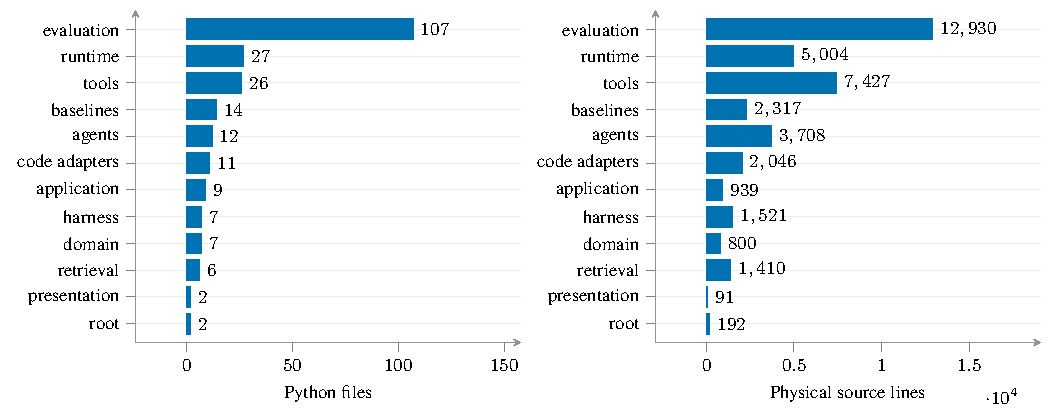
\includegraphics[width=\textwidth]{figures/code_footprint.pdf}
\caption{代码结构的描述性清点：230 文件、38385 物理行。evaluation 的文件数最多；这说明历史实验基础设施占比，不意味着相同语义覆盖、质量或用户价值。行数包含注释和空行。}
\label{fig:footprint}
\end{figure}
\source{data/report_data.json; src/cv_agent/**/*.py}

\subsection{核心与评价的依赖隔离}
K2 已把 witness 内核迁入 \code{runtime/witness/}，契约、读取政策、追踪、资源计数、场景运行及义务分别在同一包中。生产工具依赖运行时；准备器、runner 和诊断依然归 evaluation。核心 \code{agents/tools/runtime} 不反向导入评价包；新产品的公共 CLI 子命令采用延迟导入，产品测试显式拒绝导入 evaluation。

架构边界检查覆盖显式、嵌套、类型检查和已列出的字面动态导入；它不穷尽任意生成的 import 字符串。K2 的归一化文本/AST、源码绑定及实际结果对照属于迁移验收，不能替代新产品的端到端验收。\cite{k2,acceptance}

\subsection{契约作为层间接口}
\code{Candidate} 和 \code{ValidationSubject} 建立问题对象；\code{ToolObservation} 建立产出身份；\code{AgentExpertVote} 表达研究判断；\code{ReviewResult} 表达产品交付。中间过程不能用一个自然语言状态覆盖这些职责。控制器可以判定“操作完成”，但语义内核仍可以判定 UNKNOWN；报告可成功交付，而 run 可以是 PARTIAL 或 BLOCKED。
\loc{application/; presentation/report.py; domain/; agents/workflow.py}

\section{默认产品路径：本地源码到可复核产物}
\label{sec:product}
\subsection{输入、默认行为与入口}
\cmd{cv-agent review} 接受显式源码根、一个尚不存在的输出目录，以及可选的语言、观察字节预算和上下文 grant manifest。默认语言为 Python；模型、planner、Jev、多专家、quorum、early stop、执行见证、scratch 和 native build 均不属于默认必经环节。

\begin{lstlisting}[caption={默认静态入口；路径由使用者明确选择，输出目录不得已经存在。}]
uv run --no-sync cv-agent doctor /path/to/authorized/source
uv run --no-sync cv-agent review /path/to/authorized/source \
  --output /path/to/new-review-run
\end{lstlisting}
完成返回 0；PARTIAL、BLOCKED、FAILED 或 CANCELLED 返回 2。已有输出目录被拒绝，历史文件不覆盖；不可用输出或配置参数本身产生结构化错误。分析已登记的事实可在内部失败或取消时继续交付。

\subsection{服务编排和静态能力选择}
应用先运行预检，再以原始字节清单建立源码身份，复用 \code{discover_python_repository} 发现候选。候选身份从源码操作位置派生，不从期望标签或 corpus 映射派生。针对权限 mode、命令构造和动态求值选择现有对应工具，其余性质仅运行静态线索检查。

每次调用使用已有 \code{ToolRegistry}、\code{ModelToolCall} 数据协议和精确 candidate subject；工具观察的完整序列化封装包含 producer、状态、subject、引用与内容。可投递预算不足时保留私有生产者结果和公开缺口；归并只使用可接纳观察。默认工具物理执行计数为 0，因为这里的检查是静态/AST 分析，不是目标进程运行。

\begin{pseudocode}{alg:product}{离线产品审查的确定性主链}
\Pinput{授权源根 $R$；新产物目录 $O$；profile；预算 $B$；可选显式行区间 grants。}
\Poutput{版本化 ReviewResult、人工报告、私有观察与完成记录。}
\Pstep{检查源、语言和 profile 能力；失败写出 BLOCKED 诊断，不尝试 provider。}
\Pstep{边界读取源字节；保存可读/解析失败分母；建立文档、符号和中性候选。}
\Pstep{封存源/分析身份；建立初始准入视图，并对显式扩展逐项核验与收费。}
\Pstep{\textbf{for each} 源码候选 $c$，构造 $J_c$，选择已注册适用静态工具。}
\Pstep{\quad 若候选 span 不准入或能力缺失，登记缺项；不删除该候选。}
\Pstep{\quad 否则运行有限控制任务；保存原始观察和独立 producer ID。}
\Pstep{\quad 完整封装按共享 byte pool 投递；失败时保留 UNKNOWN 及实际费用。}
\Pstep{\quad 从全部相关受信观察确定性质状态；绑定源/分析身份及 evidence refs。}
\Pstep{取消停止后续调用；已完成性质事实保留，未处理分母明确。}
\Pstep{核对计数、证明和引用；在同一 staging 目录生成 JSON 和 Markdown。}
\Pstep{原子提交两份公共产物；保留权限为 0600 的私有原始观察。}
\end{pseudocode}
\loc{application/service.py; application/preflight.py; presentation/report.py}

\subsection{运行、性质、验证和任务控制状态}
产品运行状态为
\begin{equation}
r\in\{\text{COMPLETED, PARTIAL, BLOCKED, FAILED, CANCELLED}\},
\end{equation}
性质状态为
\begin{equation}
z\in\{\text{SUPPORTED, REFUTED, UNKNOWN, CONFLICT}\}.
\end{equation}
原工具验证状态仍为 CONFIRMED、REFUTED、UNRESOLVED；任务控制还区分 READY、WAITING\_INPUT、BLOCKED、FINISHED 和 FAILED。这四组状态回答“运行怎样结束”“性质依据怎样”“验证器怎样表述”“当前操作能否推进”。FINISHED+UNKNOWN 不等于失败，更不等于安全。

\begin{table}[htbp]\centering
\begin{tabularx}{\textwidth}{L{28mm}L{33mm}Y}
\toprule 组合 & 合法解释 & 边界\\\midrule
COMPLETED + UNKNOWN & 静态检查完成，性质仍未建立 & 不把弱线索升级。\\
PARTIAL + REFUTED & 某候选有充分有限否定，其他工作未完 & 不抹掉已登记证明，不宣称整个 run 完整。\\
BLOCKED + UNKNOWN & 输入或能力使本次工作不能推进 & 零候选计数可能表示未做 inventory，而非“没有问题”。\\
CANCELLED + 混合状态 & 保留先前事实，后续工具不启动 & 未处理候选仍留在分母。\\
任意 run + CONFLICT & 同身份同完整范围充分证明互斥 & 要求核对 producer，不靠专家信心消解。\\
\bottomrule
\end{tabularx}
\caption{状态分离的实例。schema 检查 20 个独立组合和不可接受的引用、计数与能力组合。}
\end{table}

\subsection{输出字段、分母与可追溯性}
\code{FindingView} 包含候选、subject、版本化性质契约、性质状态、事实、缺项、下一步和引用。\code{ReviewCounts} 分别保存源文件、解析成功/失败、候选、完成静态验证、充分性质证据、未处理候选和文档准入数量。\code{ReviewAccounting} 将工具调用、物理执行、观察/context 字节与分阶段墙钟分开。

\code{application_security} 固定 NOT\_ASSESSED，公共入口与远程权限标志固定 false。源码文本和凭据值不直接复制到公共报告；原始工具内容和内部异常保存在 \code{.private/observations.jsonl}，与 producer、内容 SHA-256 和交付状态对应。声明路径和范围本身仍是公共信息。

\subsection{原子产物与计时的精度}
JSON 与 Markdown 在同一个临时目录中写入、flush/fsync，再用目录 rename 提交。产物指向同一 \code{ReviewResult}，presentation 不创建新证明。\code{accounting.output_seconds} 记录最终提交前的准备范围；提交结束后的实际输出墙钟在私有 completion receipt 中，避免自引用计时造成虚假精度。CLI 进程时间还包括启动、导入、输出和返回，不等同内部分析时间。

\subsection{能力声明的真实边界}
默认静态 capability AVAILABLE 只说明相应工具可调用，不说明当前候选已被证明。Python 之外的产品 inventory 当前 BLOCKED，虽然研究适配器保留其他语言。模型配置存在性只检查环境键名，不读取值或 probe provider。未注册的 owned fixture check 不能执行；显式注册的无害功能检查缺依赖时只阻塞对应能力。\cite{productguide}

\section{数据契约、快照与四种身份}
\label{sec:identity}
\subsection{从结构合法到事实稳定}
Pydantic 的冻结模型约束字段赋值，但字段内部的可变容器仍可能由外部别名修改。修复前，将同一个嵌套字典交给候选、文档或 subject 后再修改该字典，可以改变已建立的语义身份。这是已复现的程序缺陷，不是抽象风险。当前 \code{SnapshotModel} 对构造和 \code{model_copy} 的嵌套字典、列表封存，并对公开读取返回深复制。\code{Candidate}、\code{CodeDocument}、\code{ValidationSubject} 和 \code{ToolObservation} 继承这一行为。普通 JSON 类型和原有序列化摘要保持兼容。

这一保证适用于声明的公共数据接口。它没有将同进程 Python 对象变成能抵抗任意反射、私有 \code{__dict__} 修改或内存篡改的安全容器。其他 \code{FrozenModel} 的字段赋值限制也不能自动解释为任意嵌套对象深层不可变。回归用例分别覆盖外部输入别名、公开读取、复制更新和源码身份的正反控制。
\loc{domain/types.py::SnapshotModel; domain/evidence.py; application/identity.py}

\begin{longtable}{L{38mm}L{111mm}}
\caption{跨研究与产品路径的核心数据对象。}\\
\toprule 对象 & 含义与权威边界\\\midrule\endfirsthead
\caption[]{（续）}\\
\toprule 对象 & 含义与权威边界\\\midrule\endhead
\code{Candidate} & 中性候选身份、仓库、路径、行号、query、性质、范围、输入和前提；标识不编码期望标签。\\
\code{CodeDocument} & 源码切片及解析结构：定义、调用、导入、路由、别名和重绑定；解析能力不等于动态语义覆盖。\\
\code{ValidationSubject} & 候选、源码索引摘要、位置、性质、范围和前提的共同证明对象。\\
\code{ToolObservation} & 原始工具状态、内容、引用、元数据、验证状态和 subject；仅生产者声明的有界语义可参与准入。\\
\code{EvidenceReceipt} & 产品的投递、原生产者、内容摘要、方法、覆盖范围与身份回执；保留原验证器状态。\\
\code{FindingView} & 性质契约、四值状态、事实、证据引用、缺项及下一步；应用安全固定未评估。\\
\code{ReviewResult} & 同一次运行的身份、finding、能力、诊断、范围准入、分母、费用与产物引用。\\
\code{AgentExpertVote} & 研究专家的标签、置信度、验证状态、引用角色、轨迹和用量；经过准入后才能投票。\\
\code{AgenticVerdict} & 研究的最终路径、最终票、原始任务执行、阻塞、检索准入、共享观察计数和总用量。\\
\bottomrule
\end{longtable}

\subsection{旧 subject 摘要与产品字节身份同时保留}
研究与已有 fixture 共用的 \code{candidate_subject(index,candidate)} 对按路径排序的文档模型作规范 JSON 序列化，计算 SHA-256。它覆盖被索引的文本和元数据；适配器提供的 \code{source_sha256} 也参与摘要。Java 方法文档包含完整文件摘要；其他格式不因此自动获得同样的完整文件保证。修复没有静默替换这个历史算法。

新产品另外定义以下身份，避免将源码内容、分析规则、执行环境和可见上下文混成一个摘要：
\begin{align}
H_s &= H(\texttt{source-bytes-v1},\operatorname{sort}\{(p,H(\operatorname{bytes}(p)))\}),\\
H_a &= H(\texttt{analysis-contract-v1},\text{profile, contracts, rules, budgets, code, parser}),\\
H_e &= H(\texttt{approved-execution-v1},\text{trusted environment manifest}),\\
H_v &= H(\texttt{retrieval-view-v1},\operatorname{sort}\{(p,l_0,l_1)\}).
\end{align}
$H$ 的实现是带算法名的规范 JSON SHA-256；非有限浮点数被拒绝。$H_s$ 使用授权根内 Python 文件的完整原始字节，编码差异、helper 与 import 所在文件的变化都能改变清单；不可读取文件的摘要显式为 null，并通过诊断说明。路径要求规范根相对形式，拒绝绝对路径、父目录跳转和反斜线别名。

$H_a$ 将分析实现和实际 Python、parser、Pydantic 版本纳入绑定，同时包含 profile、性质契约、规则及预算/排除政策。它绑定的是分析所依赖的实现范围，不是整个 Git 仓库的提交哈希。全仓源码清单另在报告数据中保存。默认静态产品 $H_e=\mathrm{null}$；有一个执行环境摘要函数不表示当前产品启用了执行。扩大获准行范围可以改变 $H_v$，在源码和分析配置相同时保持 $H_s,H_a$ 不变。

\begin{table}[htbp]\centering\small
\begin{tabularx}{\textwidth}{L{35mm}L{40mm}Y}
\toprule 变化 & 必须失效的身份 & 不应作出的推断\\\midrule
同一文件字节、helper 或 import 改变 & 源码字节身份 & 路径相同不表示证据仍有效。\\
分析规则、实现、parser 或预算改变 & 分析契约身份 & 工具名相同不表示语义相同。\\
获准行范围增加 & 视图版本 & 可见 helper 不表示已绑定运行时 callee。\\
可信环境清单改变 & 执行身份（如启用） & 静态结果不建立执行环境证明。\\
增加 citation 别名或专家角色 & 不增加原生产者 & 引用数量不表示独立证据数量。\\
\bottomrule\end{tabularx}
\caption{身份变化与失效关系。行范围和分析身份的分离以分析配置不变为前提。}
\end{table}

\subsection{结果构造阶段的交叉检查}
\code{ReviewResult} 拒绝重复 finding 和 observation 引用，校验候选分母、充分证据数量与性质状态，并要求强状态的回执匹配当前产品源码与分析身份。\code{FindingView} 的候选、subject 和性质契约必须一致；契约必须等于当前注册版本。缺引用、错误 source、错误 analysis、非法计数和手写强状态都不能只凭 JSON 格式合法通过。

这些检查将身份约束从工具调用点延伸到最终产物，降低 presentation 或外部消费方误组装结果的可能性。它们不能证明生产者实现没有缺陷；生产者的有界语义还需要回归控制和独立审查。\citep{contract,productguide,acceptance}

\section{性质契约与全局证据归并}
\label{sec:reduction}
\subsection{性质、范围和量词先于结论}
一个结论应回答明确的性质 $P$，并声明输入域、前提 $\Gamma$、范围 $\Omega$、量词及允许的证明方法。当前权限性质检查所选 mode 是否包含 others-write 位；命令性质关注已建立的可控输入是否能改变声明消费边界的语法或可执行选择；动态求值性质限定在获准函数切片和内建绑定的有界模型中。授权性质必须有主体、资源、动作与政策。这些契约均排除应用整体安全、公共入口可达性和远程权限。

未注册性质只能留下 source-derived review lead，不能因为规则名称听起来像漏洞就得到 SUPPORTED。性质正向证据通常是存在性证明；范围有限的否定事实不能外推到未检查输入或应用整体。当前系统对范围包含关系采用规范字段精确匹配，不通过自然语言判断一个局部范围是否足以覆盖更大范围。

\subsection{完整投递是强结论的必要条件}
对原生产者观察 $o$，定义证明资格 $Q(o,J)$：
\begin{equation}\begin{aligned}
Q={}&\operatorname{exactSubject}\land\operatorname{identityBound}\land\operatorname{ok}\\
&\land\operatorname{completeDelivery}\land\operatorname{candidateCoverage}\\
&\land\operatorname{supportedMethod}\land\operatorname{materialStatus}.
\end{aligned}\end{equation}
\code{source_pattern} 和 \code{source_read} 不属于充分证明方法。生产者私有完整结果存在，而公共证书被截断、抑制、预算拒绝或未投递时，公共结果仍不能升级。error、blocked 和局部观察可提供诊断，但不作为同候选完整证明。

命令检查是一个需要保留双层状态的例子。原 \code{inspect_command_construction} 观察仍可报告 \code{UNRESOLVED}；共享准入逻辑在严格的输入控制、消费语义、绑定及完整范围条件下，能够建立有界静态性质结论。产品单独记录 \code{accepted_static_status}，不改写原验证器状态，也不把静态分析改称执行见证。该投影只允许注册命令工具、特定方法和性质组合。

\subsection{原生产者去重与四值归并}
归并按原 producer ID 去重。忽略展示 citation，并将生产者拥有的 \code{evidence_ids} 规范为去重排序集合；helper/source 引用的内容保留。相同 producer ID 对应不同事实是协议错误。同一证书被三名专家引用仍是一个原观察；两个不同 producer ID 也不自动保证统计独立。

设 $S^+=\{o:Q(o,J),v(o)=\mathrm{CONFIRMED}\}$，$S^-=\{o:Q(o,J),v(o)=\mathrm{REFUTED}\}$，则
\begin{equation}
z(J)=\begin{cases}
\mathrm{CONFLICT},&S^+\ne\varnothing\land S^-\ne\varnothing,\\
\mathrm{SUPPORTED},&S^+\ne\varnothing\land S^-=\varnothing,\\
\mathrm{REFUTED},&S^+=\varnothing\land S^-\ne\varnothing,\\
\mathrm{UNKNOWN},&S^+=\varnothing\land S^-=\varnothing.
\end{cases}
\end{equation}
充分证明相互矛盾时显式 CONFLICT；新的无关 UNKNOWN 不覆盖已存在的充分证明。这里的顺序不敏感成立于同一组规范观察，不意味着生产者发现新事实之前系统已知道该事实。

\begin{pseudocode}{alg:reduce}{确定性的候选性质归并}
\Pinput{精确 subject、注册性质契约、当前身份、已交付观察集合}
\Poutput{四值性质状态、原生产者回执、事实与缺项}
\Pstep{对每个观察检查 subject；不同 subject 不进入该候选的证明集合。}
\Pstep{去除展示 citation；规范引用集合；以原 producer ID 去重。}
\Pstep{若同一 producer 对应不同规范事实，显式报告协议错误。}
\Pstep{按 producer ID 排序，构造内容摘要、方法、覆盖范围、投递和身份回执。}
\Pstep{保留原验证器状态；仅为注册命令静态逻辑计算独立的准入投影。}
\Pstep{只对满足 $Q(o,J)$ 的回执收集正向与否定证明。}
\Pstep{依据 $S^+,S^-$ 输出 SUPPORTED、REFUTED、UNKNOWN 或 CONFLICT。}
\Pstep{保留不充分观察的事实、缺项与建议；应用安全状态固定 NOT\_ASSESSED。}
\end{pseudocode}
\loc{application/evidence.py::reduce_observations; domain/product_result.py}

\subsection{研究路径的晚到证据重新准入}
修复前，研究专家票可能在早期通过准入；后续相关矛盾观察到达后，最终投票仍使用既有票。当前 \code{global-evidence-v2} 在 slow adjudication 和 fast 判断前，以所有\emph{已经实际投递}的相关任务轨迹重新检查各实质票。证据不足导致该票降为 ABSTAIN；非法协议和其他内部错误继续显式传播。原始模型提案、任务记录、观察和成本保留。

\begin{pseudocode}{alg:global}{研究最终票的全局重新准入}
\Pinput{固定时点的最终专家票与所有已收到任务轨迹}
\Poutput{用于本次 slow/fast 判定的合法票集合}
\Pstep{建立候选和性质一致的全局已投递证据上下文。}
\Pstep{对每张 VULNERABLE/SAFE 票重跑原准入规则。}
\Pstep{若仅发生 InsufficientEvidenceError，保留原提案并将当前票降为 ABSTAIN。}
\Pstep{若发生协议、身份或内部错误，显式失败，不伪装成语义 UNKNOWN。}
\Pstep{用重新准入后的票计算 quorum 或固定票早停条件。}
\end{pseudocode}
\loc{agents/evidence_policy.py; agents/workflow.py}

E5 的 guarantee 仍限于固定、实际已知票集合的判决不变性。尚未取到的未来证据没有被量化或穷尽，因此不能声称早停能保证后续永不出现矛盾事实。产品路径没有专家投票和早停，直接归并全部已投递静态结果。\citep{acceptance,contract}

\section{任务控制、上下文扩展与证书投递}
\label{sec:delivery}
\subsection{控制完成与验证完成分别建模}
产品的 \code{TaskController} 接受拓扑有序的任务和真实数据依赖，区分 READY、WAITING\_INPUT、BLOCKED、FINISHED 和 FAILED。准备观察、环境预检、工具运行完成、验证器完成、性质证明和整个运行完成是不同事实。验证器合法返回 UNRESOLVED 可以完成协议并解锁依赖，但不提供充分证明。准备成功或 error 不能冒充完成验证器。

可选能力不可用时只阻塞依赖它的任务；独立静态任务继续运行。显式补充输入后重新检查等待及依赖，不凭重试次数猜测前提已满足。无效动作默认最多两次；研究任务图另有显式递归上限 16。受控测试实际执行八个计划任务，并对注入的无进展循环验证有限终止。这些数值约束调度，不证明选中的任务具有高价值。

\begin{figure}[htbp]\centering
\begin{tikzpicture}[node distance=7mm]
\node[smallbox] (ready) {READY};
\node[smallbox,right=12mm of ready] (wait) {WAITING\_INPUT};
\node[smallbox,right=12mm of wait] (blocked) {BLOCKED};
\node[smallbox,below=14mm of ready,fill=green!8] (finished) {FINISHED\\可为 UNKNOWN};
\node[smallbox,below=14mm of wait,fill=warm!8] (failed) {FAILED\\协议 / 内部错误};
\draw[arrow] (ready)--node[above,font=\scriptsize]{缺业务输入}(wait);
\draw[arrow] (wait)--node[above,font=\scriptsize]{依赖不可用}(blocked);
\draw[arrow] (ready)--node[left,font=\scriptsize]{合法返回}(finished);
\draw[arrow] (ready.east)--++(3mm,0)|-node[pos=.8,above,font=\scriptsize]{异常}(failed.west);
\draw[arrow] (wait.north) to[bend right=45] node[above,font=\scriptsize]{显式补充后重检}(ready.north);
\end{tikzpicture}
\caption{任务控制态概念图。状态恢复依赖显式输入和能力检查；性质状态由证据归并另行计算。图展示主要转换，不列出全部实现分支。}
\end{figure}
\loc{application/controller.py; agents/workflow.py; harness/defaults.py}

\subsection{行范围视图与事务性扩展}
\code{SourceReadView} 的授权单位是规范路径和闭区间行号。完整源码清单属于使用者选择的授权根；默认静态索引可内部解析支持文件，但内部解析不是免费模型上下文投递。限定初始范围时，工具只拿到已准入切片。路径相同也不能免费读取另一个行区间。

扩展要求显式 reason、授权清单成员、行范围合法以及重新读取后的字节摘要一致。完整扩展封装按 UTF-8 计费，包含标识、元数据和 JSON 外壳；只有成功投递后才改变视图版本。预算拒绝、源码漂移或越界读取保持原视图。重复投递同一上下文也记账。获准看到 helper 源码之后，仍须建立调用绑定，才能将 helper 语义用于候选证明。

\begin{pseudocode}{alg:context}{先投递、后准入的上下文扩展}
\Pinput{当前视图 $V$、显式 $(p,l_0,l_1,\mathrm{reason})$、授权清单、上下文预算}
\Poutput{更新后的视图与准入回执，或保持原视图的拒绝诊断}
\Pstep{验证规范路径、正行区间、清单成员和明确的扩展理由。}
\Pstep{通过既有安全源码读取边界读取，不跟随符号链接；重核文件字节摘要。}
\Pstep{将请求切片与元数据序列化为完整封装 $s$，计算 $b=|\mathrm{UTF8}(s)|$。}
\Pstep{若 $b$ 超过剩余预算，输出 REJECTED；不改变 $V$。}
\Pstep{成功扣减 $b$ 后将该行区间加入 $V$，计算新的 $H_v$。}
\Pstep{留下 ADMITTED 回执；不改变源码字节身份，也不宣称运行时调用关系已成立。}
\end{pseudocode}
\loc{application/context.py; code_adapters/source_files.py}

\subsection{共享池与最小证书预留}
产品默认观察池 $B=8192$ 字节，独立诊断预留 $D=256$ 字节。\code{allocation_plan} 支持声明各必需证书已验证的最小尺寸 $m_i$；计划可行需满足
\begin{equation}
\sum_i m_i+D\le B.
\end{equation}
一次投递证书 $c_i$ 之前，还须保护其他尚未投递必需证书的预留：
\begin{equation}
|c_i|+\sum_{j\ne i,\,j\notin\mathrm{delivered}}m_j\le B-D-B_{\mathrm{used}}.
\end{equation}
\textbf{当前产品服务没有必须证明成功的义务，实际传入的 \code{minimum_bytes} 是空映射。}预留接口及其正反控制已验收，不应据此声称服务已预测所有语义证明的最小长度。无法投递完整证明时，原结果保留在私有账本，公共 finding 维持 UNKNOWN，运行可形成 PARTIAL。

受控证书反例使用四个完整 JSON 证书，尺寸为 2500、1000、1000、1000 字节。简单平均四分先给第一个任务 2048 字节，短缺 452 字节；共享池在保留 256 字节诊断之后仍可容纳全部 5500 字节，余额 2436 字节。该反例说明平均分配可能拒绝一个总体可行计划，\emph{不证明任意实际工作负载的性能改善}。冻结的研究 E 系列累计均分政策保留，不将产品政策回填为历史实验配置。
\begin{figure}[htbp]\centering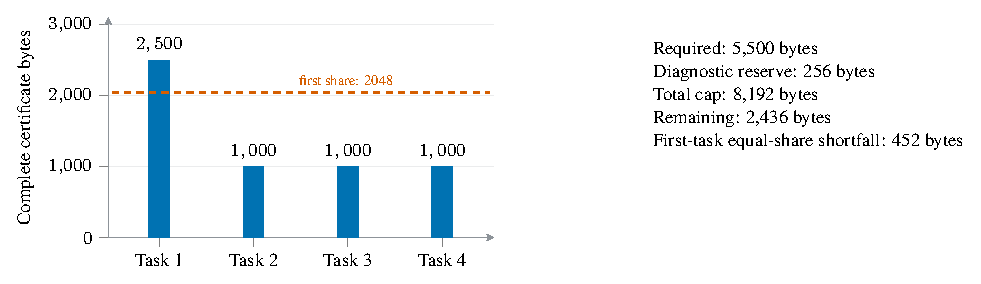
\includegraphics[width=\textwidth]{figures/certificate_budget.pdf}
\caption{完整证书分配的确定性数值反例。单位是实际序列化 UTF-8 bytes，不是 provider tokens；数据来自 A22/A24 受控投递测试。}\label{fig:certificate}
\end{figure}

\begin{pseudocode}{alg:certificate}{原生产者缓存与完整证书投递}
\Pinput{producer ID、不可变完整 bytes、全局池及必需预留}
\Poutput{投递回执或明确预算拒绝}
\Pstep{缓存原 producer 的完整 bytes；相同 ID 但不同 bytes 是协议错误。}
\Pstep{计算本次完整尺寸及其他未投递必需证书预留。}
\Pstep{若无法完整容纳，不发布证明资格；保存私有结果和诊断。}
\Pstep{否则按完整 bytes 计费，生成新的 delivery ID 并保持原 producer ID。}
\Pstep{重投递同一缓存仍扣 bytes；不再次调用生产者，不增加物理执行数。}
\end{pseudocode}
\loc{application/delivery.py; application/service.py}

\subsection{私有观察与原子产物提交}
产品的公共 JSON 与 Markdown 省略源码正文和凭据值；业务 reason 中带标签的秘密在展示时脱敏。文件名、位置和范围仍属于报告信息。原始工具观察及内部异常保存在 \code{.private/observations.jsonl}，文件 0600、目录 0700；内容摘要和引用追溯到原账本。展示脱敏不修改源码身份。

公共 JSON、Markdown 和私有目录在同一 staging 目录准备，原子重命名到尚不存在的最终目录。取消索引或工具阶段时，已登记事实保留，后续工具不再启动。工具内部失败留下私有异常类别与 traceback，而不是丢弃先前充分证据。配置和输出目录本身不能使用时返回结构化 CLI 错误，不覆盖既有目录。

\code{accounting} 分别记录准备、分析、gate、模型及产物准备耗时。JSON 序列化前无法精确知道最终提交总耗时；\code{.private/completion.json} 因而另记包含提交阶段的输出墙钟。默认产品 gate/model 均为零。私有目录权限是本地访问保护，原子提交是产物一致性机制，两者都不构成完整主机隔离证明。\citep{productguide,acceptance}

\section{源码发现、适配与 Code-RAG}
\subsection{仓库级候选发现}
\code{discover_python_repository} 以确定性的路径顺序遍历 Python 文件，排除版本库、虚拟环境、依赖和构建目录；通过源码读取边界读取字节，记录文件 SHA-256，检测编码并解析函数切片。同时增加完整模块文档，用于保留导入时操作和类体。

\code{StaticScanner} 根据 AST 调用、已解析别名、路由装饰器和有限规则，生成命令执行、动态求值、数据库操作、模板操作、权限 mode、授权边界、动态属性和进程控制等候选。重叠模块与函数切片按最小适用 span 去重。稳定候选标识由仓库、源文件、行号和规则生成，标识不是期望标签。

解析失败作为清单的一部分保留，不从分母中静默消失。扫描报告明确 \code{discovery_is_validation=false}。一些 pilot 明确采用有限候选前缀；这属于被记录的实验选择，不能被说成全仓所有候选已审查。源码发现、位置匹配、候选标签判断和运行时见证必须分别统计。
\loc{agents/discovery.py; agents/scanner.py; evaluation/discovery.py}

\subsection{多语言解析层级}
Python 适配器基于 AST 保存函数范围、调用、导入别名和模块绑定；Java、JavaScript/TypeScript、Go 使用对应解析支持构造文档与调用元数据。对不具有相同语义覆盖的格式，系统保留显式 fallback 文档。

\begin{table}[htbp]
\centering\small
\begin{tabularx}{\textwidth}{L{32mm}Y}
\toprule 层级 & 实际提供的信息及限制\\\midrule
Python AST & 函数与方法切片、别名与调用元数据；部分有界值、数据流、命令和权限语义。\\
Java 解析 & 方法文档、调用、完整原文件摘要与有界项目夹具；不代表一般 Java 应用验证。\\
JS/TS 与 Go 解析 & 定义、形式参数、调用和路由等结构；当前非 Python flow 仍包含有限逐行近似。\\
Fallback & 文件级或文本级的 imports、配置、轨迹相关上下文；不得报告为完整 AST 调用图或深层语义证明。\\
\bottomrule
\end{tabularx}
\caption{适配器层级说明。解析能力与漏洞证明能力是两个不同维度。}
\end{table}

源文件读取使用相对目录描述符并拒绝符号链接，包括路径中的链接父目录。这样可以阻止普通索引步骤通过 symlink 越出源码树。这个读取约束不替代执行环境中的资源与文件系统隔离。
\loc{code_adapters/source_files.py; code_adapters/repository.py}


\Needspace{6\baselineskip}
\subsection{文档索引和图构造}
\code{RepositoryIndex} 拒绝重复文档路径，保存源码词频、路径词频、定义表、前向及反向调用边。图边必须根据已知限定名、导入别名和源文件关系建立；已知外部调用不得连接到无关的同名本地函数。一个图邻居表示检索候选关系，不自动证明动态调用可达。

检索支持 local、text、graph 和 hybrid。graph 在声明方向上进行有界遍历，再按词法相关性或距离排序；\code{both} 模式保留前向路径优先信息。直接解析出的相关 callee 可以优先准入，并记录跳过原因、调用来源、符号、图距离和文档摘要。
\loc{retrieval/index.py; retrieval/context.py; retrieval/dependencies.py}

\subsection{默认文本评分与 BM25 诊断}
保留研究路径的默认文本排序是 TF-IDF 风格的词法评分。设查询词次数为 $q_t$，文档词频为 $f_{t,d}$，文档总数为 $N$，文档频率为 $df_t$，基本项为
\begin{align}
\operatorname{idf}(t)&=\log\frac{N+1}{df_t+1}+1,\\
s_{\mathrm{text}}(q,d)&=\sum_{t:f_{t,d}>0}q_t\,(1+\log f_{t,d})\,\operatorname{idf}(t).
\end{align}
路径形式的查询还加入路径词、完整路径子串和路径片段加权。这些都是可复核的词法启发式。

\code{MetadataBM25Index} 是独立的增强词法诊断，使用源码、路径和符号，代码常数对应 $k_1=1.2$、$b=0.75$。它没有替换冻结的默认 E2。旧概述把所有文本检索都简称 BM25 时，本文以实际实现为准。
\loc{retrieval/index.py::_lexical_scores; retrieval/bm25.py}

\subsection{同一局部基底与图、文本增强}
所有系统先取得同一候选局部文档。增强结果经过确定性的去重、数量上限与上下文裁剪，避免扩大一个系统的隐藏取证范围。对于较长代码，context 模块可围绕候选、源、sink 及赋值依赖保留局部窗口，并显式标明非相邻上下文省略。

hybrid 将候选出发的图检索、文本检索及词法 seed 出发的图检索按分支上限合并，再受共享文本预算限制。因此，hybrid 的 \code{top_k} 是分支限额，其联合条数语义与普通 text/graph 的全局条数限额不能混为一谈。与不同检索方法比较时应同时报告实际文档数和序列化预算。

\subsection{两层文本预算与 API 用量}
旧的确定性实验使用词法上下文单位；当前 agent 对模型可见的序列化文本使用 UTF-8 字节上界。对完整序列化载荷 $s$，计数为
\begin{equation}
B(s)=|\operatorname{UTF8}(s)|.
\end{equation}
它将候选投影、引用、路径、JSON 转义和内容一起计入相应文本预算。裁剪是在完整序列化后判定能否容纳，长标识符不会被当作一个免费单位。

此计数不是模型服务商的精确 tokenizer 计费。系统指令、工具 schema、历史消息、规划和输出还会增加实际请求 tokens。检索预算、观察预算与 provider usage 应分别记录。

\begin{table}[htbp]
\centering\small
\begin{tabularx}{\textwidth}{L{48mm}L{26mm}Y}
\toprule 通用 E 系列默认项 & 默认值 & 语义\\\midrule
候选局部基底 & 4096 & 模型可见序列化文本的上界单位。\\
增强上下文 & 12288 & E2--E5 的声明增强预算；E1 为 0。\\
增强条数 & 12 & 普通文本/图检索的默认 top-k。\\
图距离上限 & 4 & E3--E5 默认最大跳数。\\
ReAct 步数 & 8 & 一次任务循环的最大模型步数。\\
工具观察预算 & 8192 & 同一专家多个子任务累计共享。\\
规划子任务上限 & 8 & 计划的有限规模约束。\\
任务图递归上限 & 16 & 显式业务流程上限；控制无进展循环。\\
\bottomrule
\end{tabularx}
\caption{默认值来自 Harness；专项 profile 可声明不同策略，报告实验时必须使用其实际配置。}
\end{table}
\loc{harness/defaults.py; retrieval/tokens.py; agents/workflow.py::_bounded_context_prompt}

\subsection{模型投影与路径准入}
初始模型上下文仅包含显式候选投影及被选中的检索文档。候选投影包含中性身份、仓库、路径、行号和明确的性质、分析范围；私有 query 与任意 caller metadata 不直接复制给模型。

工具作用域的 admitted paths 来自最终实际投递的文档集合。工具可以重读、搜索或遍历其中已准入的路径，但不能将 local 系统扩成全仓检索。证据路径准入只约束 agent 的取证范围；见证内核执行目标时另有真实源码闭包绑定与文件系统读取准入，二者的用途不同。


\subsection{产品与研究取证范围的关系}
产品默认只接受 Python 本地源码，研究适配器的多语言结构能力没有被自动纳入产品能力承诺。新 SourceReadView 的行区间扩展与研究 admitted paths 是两种声明边界；旧 E 系列的上下文预算和检索定义保持冻结。第\ref{sec:delivery}节的扩展机制不能用来解释历史 E1 已经具备全仓取证。

\section{研究系统变体、计划与 ReAct}
\subsection{E1--E5 的受控差异}
\begin{table}[htbp]
\centering\small
\begin{tabularx}{\textwidth}{L{12mm}L{23mm}L{18mm}L{42mm}Y}
\toprule 系统 & 检索 & Planner & 专家 & 最终规则\\\midrule
E1 & local & 关闭 & scan & 单票\\
E2 & text & 关闭 & scan & 单票\\
E3 & graph & 关闭 & scan & 单票\\
E4 & graph & 开启 & scan、taint、authz & 完整 quorum\\
E5 & graph & 开启 & scan、taint、authz & 前两张最终票可尝试早停；否则完整 quorum\\
\bottomrule
\end{tabularx}
\caption{当前 E 系列默认定义。真实运行使用独立声明的模型与实验配置。}
\end{table}

V1--V5 是保留的确定性开发基线，其专家规则、预算和输出不等同 E 系列真实模型循环。V 系列、synthetic 和 scripted 结果用于机制对照，不能充当 live 模型结果。

\subsection{三种专家职责}
scan 检查源码结构、候选操作和适用的受控验证；taint 分析输入到消费边界的来源、传递、转换与缺边；authz 分析主体、动作、资源或租户、守卫与执行位置。不同任务允许的工具来自各自 Harness，不能让一个不适用专家为了凑票而强行输出实质判断。

各专家可以共享被合法投递的依赖观察，但必须自行形成结构化结论。专家角色不同不意味着其数据或证据统计独立。共享见证的票数和原始见证观察数在结果中另行记账。

默认 E4/E5 使用固定专家集合。可选 \code{applicable_v1} 将适用性表示为 applicable、not applicable 或 undetermined；明确计划任务仍必须执行，未能排除的专家仍保留。可选政策不会降低 quorum：适用专家不足两名时返回弃权。它是单独实验选项，不能默默替换固定基线。
\loc{harness/defaults.py; agents/applicability.py}

\subsection{类型化计划与确定性义务}
\code{ValidationPlan} 要求至少一个可执行任务，任务标识唯一，目标、专家、验证器和成功条件非空。依赖必须引用之前出现的已知任务，因此提交的计划本身具有拓扑顺序；未知和前向依赖直接拒绝。

计划不是任意自然语言待办表。policy 层推导必要验证义务：符合完整候选性质范围的 registered fixture 可以替代对应命令检查；适用见证可生成独立 witness 任务，并让后续命令分析依赖其完成；权限 mode 的必要验证义务仍单独保留。任务必须使用专家可调用且已注册的验证器。

\code{compose_plan} 将政策锁定任务和合法外部提案组合，记录 policy、jev 或 llm 来源。成功条件描述要完成的取证动作，不能被解释为已经满足了漏洞成功标准。
\loc{agents/planning.py; agents/plan_policy.py; domain/review.py::ValidationPlan}

\subsection{LangGraph 的实际执行方式}
当前图注册 retrieve、plan、scan、taint、try\_fast、authz 和 adjudicate 节点。从 retrieve 到 plan 后，由当前依赖状态选择下一节点。图不是把三名专家无条件同时启动的固定并行流程。

就绪任务需要其所有依赖的 \code{validator_completed=true}，声明专家顺序只对多个就绪任务作 tie-break。某个专家可以在其他专家执行后恢复；同一专家各子任务的中间判断都保存在 task executions，直到自身全部任务处理完，才使用最后的累积判断生成一张最终票。

\begin{pseudocode}{alg:schedule}{保留研究路径的依赖调度}
\Pinput{类型化计划、任务执行记录、专家顺序、既有同专家预算}
\Poutput{下一任务或有限终止，以及每位专家至多一张最终票}
\Pstep{从执行记录取得 validator\_completed=true 的任务集合。}
\Pstep{传播未完成的必需依赖，建立 blocked tasks。}
\Pstep{找出尚未执行且全部依赖完成的任务，按专家顺序作 tie-break。}
\Pstep{执行一个就绪 ReAct 子任务，记录观察、验证完成与累计成本。}
\Pstep{专家全部子任务处理后，生成一张累积最终票。}
\Pstep{在 fast/slow 判定前，以所有已收到相关观察重新准入实质票。}
\Pstep{无可运行任务、达到业务限额或存在必需阻塞时，按协议有限收尾。}
\end{pseudocode}

终止与验证完成分别记录。合法 ABSTAIN 可以结束一个任务，但如果必需验证器没有完成，依赖任务仍被阻塞；一个已经完成而结果为 UNRESOLVED 的验证器可满足调度依赖，却不会因此支持实质漏洞判断。有阻塞必需任务时，工作流最终弃权。
\loc{agents/workflow.py::_next_task; agents/workflow.py::_blocked_tasks}


\subsection{从模型动作到最终 JSON}
ReAct 输入包含专家 mandate、任务提示、允许工具 schema、最终输出 schema、剩余观察预算和必需验证器。每一步模型可请求类型化工具，或提交最终 JSON。工具结果经过运行时引用生成、投递裁剪及状态封装后，以 tool message 返回给模型。

最终 JSON 需要通过 schema、专家身份、引用、验证完成与证据准入检查。模型提出的 VULNERABLE 或 SAFE 不是最终获准的票；拒绝原因会作为结构化反馈进入有限的剩余循环。所有已发送模型请求仍计入用量。
\loc{agents/react.py; domain/chat.py}

\subsection{工具边界的处理顺序}
注册表首先检查剩余观察预算，再检查专家工具 allowlist、注册与可用性、输入 schema、任务绑定的 fixture ID 和重复调用。执行器只接受已注册工具及数据型参数，不提供任意模型生成 shell 命令的运行接口。

同一子任务中，相同工具名和规范化参数若已成功执行，或生产者已完成，不再次物理执行。后续重复得到 blocked 观察并指向先前引用。重复执行记忆基于\textbf{执行事实}，不能因为先前结果在投递时被裁剪而遗忘。另一个子任务有自身 scope，仍可执行其分配的验证器。

工具异常通过类型化边界变成 error 观察；错误工具身份等协议不一致则显式报错。工具调用数是尝试数，包含被拒绝或失败的调用，不能被等同成功验证次数。
\loc{tools/registry.py::invoke; runtime/journal.py::RecordedTools}

\subsection{完整观察与模型可见载荷}
生产者的完整结果和模型实际收到的结果是两个记录面。注册表对完整序列化工具响应计数，必要时结构化裁剪。截断、抑制、error 或 blocked 观察不能作为充分证明。发生截断时，传给模型的确认资格及 proof scope 被移除，原始产物则保留供审计。

观察预算耗尽后，诊断信息必须能够到达模型。当前用单独的 Harness 诊断说明预算已尽，且该说明不消耗其报告已经耗尽的预算，避免出现“空 tool message”诱发重复调用。模型随即进入不能新增工具的收尾阶段，证据门槛不降低。

\subsection{多个子任务的共享预算}
同一专家总观察预算为 $B_e$，已执行子任务保留累计用量。计划含 $n_e$ 个该专家任务时，第 $k$ 个任务的累计可用上限按任务份额开放，可概括为
\begin{equation}
 B_{e,k}=\left\lfloor B_e\frac{k}{n_e}\right\rfloor.
\end{equation}
这给后续任务保留预算，而前面未用完的份额仍可被后续使用。规划和可选 routing 也有明确计数，不作为免费上下文。该机制不保证模型会采用最有效动作，只保证已声明资源边界可审计。

\subsection{正常收尾、弃权与错误}
证据充分时可以形成实质票；经过至少一次工具尝试后可以自愿弃权；预算末尾反复坚持证据不足实质标签时，运行时按契约有界弃权，并保留 proposed label、拒绝原因及终止类型。零工具尝试且无法满足 vote schema 的执行返回显式失败或未完成，不伪造工具调用。

未知 citation、subject 漂移、非法协议、模型传输异常和内部错误不能统统归为普通“证据不足”。相反，未解析语义和可说明的预算终止需要保留具体原因，使后续分析可以区分能力、基础设施、协议和资源限制。


\subsection{新增的全局证据与任务图边界}
修复后的共享 workflow 启用 global-evidence-v2，并将 LangGraph 的业务递归上限明确设为 16。回归同时包含八个真实任务执行的正例和强制无进展循环的负例；没有将上限扩大来掩盖循环。全局准入规则见算法\ref{alg:global}。原规划义务、必需 witness 依赖、E 系列累计均分观察政策均保留；产品路径的真实数据依赖控制不被回填成原研究实验的新定义。
\loc{agents/workflow.py; harness/models.py; harness/defaults.py}

\section{静态分析器与类型化验证工具}
\subsection{命令分析的有界语义}
命令分析器使用有限抽象值结构，包括字符串片段、有限 choice、来源及安全处理信息，并维护执行路径、绑定和副作用缺口。普通未知字符串与已经建立的输入来源不同；转义只在已经解析的消费上下文中有意义。

分析按 Python 求值顺序处理已支持的赋值、参数传递、有限分支与展开 helper。确定不能成功的解包不产生正常后继；有限备选同时包含成功和失败时保留成功路径；未知迭代协议保留可能相关副作用。未知对象的 truth、比较、属性访问，以及未知函数即使返回值未使用，也不能默认纯净。

整函数候选包含实际调用链中相关的操作。未经解析的前置调用可能改变后续值、绑定或可达性时，分析不能把后面的猜测 sink 当作完整危险链。独立、已经完整建立的危险链则不因另一条无关未解析路径而被删除。

\code{inspect_command_construction} 负责将分析事实封装成范围、来源、路径和缺口记录。该静态工具保留验证状态 UNRESOLVED；其完整分析事实可按准入规则支持特定预测，但不被描述为真实应用执行见证。
\loc{tools/analysis/commands.py; tools/validation/commands.py}

\subsection{数据流与消费上下文}
\code{trace_dataflow} 在已准入文档和调用图内追踪来源、sink、sanitizer、变量及调用参数绑定。Python 主链使用 AST 表达式和分支合并；其他语言包含有限逐行近似。工具返回可能到达或尚未建立，并保持 UNRESOLVED。

一个名称像 sanitizer 的调用并不证明防护有效。消费上下文改变、后续原始片段追加、解释器消费参数或输入、容器修改和未知转换，都需要重新核对。非 shell argv 和 shell 参数转义是不同的性质事实，不能仅凭 \code{shell=False} 字样给出宽范围 SAFE。
\loc{tools/analysis/python_flow.py; tools/analysis/sanitizers.py; tools/validation/dataflow.py}

\subsection{权限 mode 验证}
\code{validate_permission_mode} 对有界声明的 chmod mode 性质执行静态语义检查。受支持的常量和路径条件可以产生匹配的 CONFIRMED 或 REFUTED，但相关未解析副作用、绑定变化、未知对象协议和范围失配仍保持未决。

不同资源的权限设置不能彼此抵消；先宽后窄不能证明不存在时间窗口。一个明确调用的位模式证明不覆盖完整目录竞态，也不覆盖整个函数的授权安全。工具在产生实质状态时核对位置、输入前提和 \code{chmod-mode-others-write} 性质，消费端再次核对。
\loc{tools/validation/permissions.py}

\subsection{动态求值的 AST 探针}
\code{probe_python_eval} 是有界 AST 解释器的输入控制检查。它在准入的 Python 切片和调用跳数内处理有限参数、常量、局部赋值、分支与返回，具有 256 步解释上限。它不会执行仓库 Python、导入目标模块或调用任意宿主函数。

该工具需要确认具体输入到同一 builtin eval 参数的关系；builtin shadowing、未知外部调用、装饰器、参数展开或未支持构造保持 UNRESOLVED。CONFIRMED 是声明模型下的函数切片见证，不能被扩成完整应用执行或远程输入权限证明。
\loc{tools/analysis/python_probe.py; tools/validation/probes.py}

\subsection{授权事实、差分与 registered fixtures}
授权工具提取主体、动作、资源范围、ownership 比较和路由/服务守卫。参数名或不明上游策略不是具体授权证明；没有找到守卫不等于已建立绕过。源码 diff 可以描述两版变更，不能自行确认漏洞或补丁安全。

registered fixture 声明其 subject 和 proof scope，包括性质、candidate/local 覆盖、方法和支持的状态。\code{source_pattern} 方法不能作为充分候选 fixture 证明。一个不匹配的 fixture、另一个 helper 的结果，或者固定 token 夹具的成功，都不能通过通用 CONFIRMED 字段证明任意性质。

项目自有 loopback HTTP 验证比较已声明的授权与未授权响应，且只适配相应 \code{authorization-boundary} 范围。HTTP 状态码不能被注册者文字声明成命令执行或权限证明。其驱动禁用代理与重定向，应用回调置于受限子进程，网络仅保留预绑定本地 listener。
\loc{tools/validation/authorization.py; tools/validation/comparison.py; tools/validation/fixtures.py}

\subsection{执行隔离的适用假设}
受控 fixture 和 witness 使用可抛弃的 Linux 子进程，配置有限资源、截止时间、文件描述符及系统调用、文件系统访问约束；隔离不可用时拒绝执行。文件读取需要显式 read roots 或身份绑定的叶子准入；目标侧文件系统写入被禁止。

这些边界为项目拥有、明确注册的有界验证服务提供控制。源码索引、AST 探针、registered callback 与真实目标 worker 具有不同执行模型，不能笼统把它们都称为在同一个通用沙箱里运行。模型接口始终只提出 schema 允许的数据与工具调用。
\loc{runtime/fixture_isolation.py; runtime/fixture_syscalls.py; runtime/witness/isolation_policy.py}


\subsection{为何保留正例和未解析状态}
对已支持构造，完整正向和否定控制必须继续通过；对未支持构造，结果保留具体缺项。将所有分析统一返回 UNRESOLVED 虽能避免某些假确认，却会抹掉真实能力，违反测试契约。当前验收既要求拒绝错误范围、未知副作用和不匹配来源，也要求充分、匹配的已知语义仍可形成有界结论。完整 Python 异常控制流、任意动态分派和外部库语义没有因此获得完备保证。

\section{有界见证、Jev 与最终投票}
\subsection{为什么需要单独的见证接口}
静态分析遇到复杂下载、框架分派、对象状态和 helper 副作用时，扩大解释器覆盖面没有自然终点。执行见证选择另一种受限能力：固定一个已经定位的候选和一组完整分类前提，执行真实源码，核对是否在该条件下出现预期的命令消费事实。

工具名为 \code{run_bounded_execution_witness}，proof contract 为 \code{bounded-execution-witness-v1}，性质固定为 \code{command-execution}，支持状态只有 CONFIRMED。未达到确认条件时返回具体 gap 和 UNRESOLVED。它不提供 REFUTED，也不通过有限次未观察到展开来输出 SAFE。
\loc{tools/validation/bounded_witness.py; runtime/witness/contract.py}

\subsection{清单、执行上下文与准备状态}
系统从源码、subject 和可信 execution context 构造 \code{WitnessManifest}。清单包含入口及调用方式、参数、构造数据、输入位置、分类场景、解释器、目标模块库存、资源配置、对照和受控记录信息。

\code{WitnessExecutionContext} 承载 checkout、解释器、读取准入、资源和响应方式。模型不能替换这些运行时控制，也不能选择源码摘要、内核策略或证明义务。模型只能按照工具指出的缺失字段补充数据型调用信息。

缺字段时输出 \code{ValidationPreparation}，明确 \code{witness_attempted=false}、缺失字段名、目的位置、是否需要分类及继续动作。准备状态不算验证完成。对已有 dataset 场景，工具要求保留声明场景；对空场景候选，模型提出完整分类假设后才可进入执行。
\loc{tools/validation/witness_manifest.py; domain/validation_protocol.py}

\subsection{分类场景与双 subject}
每条前提包含值、分类和 rationale。分类为攻击者可控输入、部署配置或环境条件。输入参数、布尔开关、条件、值、构造数据和预置文件均使用有界数据 schema；布尔值是严格 JSON 布尔，字符串形式的布尔不能冒充真实布尔。

系统保存原始 subject，另生成 \textbf{execution subject} 表示这次场景条件。场景来源和规范 JSON 摘要分别记录。模型假设不能改写原候选身份，不能与未分类外层数据混用，也不能覆盖已有数据集场景。数据集自带的旧场景同样需要可信分类记录才能执行。

分类描述“需要谁控制哪些输入或配置”，没有证明现实部署中的远程调用权限。完整运行时核验仍要验证值、分支、构造对象及预置数据实际满足声明。当前原始观察明确保存 \code{remote_authority_established=false}。
\loc{tools/validation/witness_scenario.py; runtime/witness/scenario_runtime.py}

\begin{figure}[htbp]
\centering
\begin{tikzpicture}[node distance=7mm]
\node[wide] (draft) {候选与可信执行上下文\\系统生成清单};
\node[wide,below=of draft] (prepare) {准备检查\\分类与调用字段完整，否则返回准备缺口};
\node[wide,below=of prepare] (bind) {身份准入\\原始 / 执行 subject、源码库存与解释器};
\node[wide,below=of bind] (worker) {独立受限 worker\\执行真实入口并捕获候选进程边界};
\node[wide,below=of worker] (verify) {运行时义务 + 良性对照\\值、分支、preexec、来源与受控重放};
\node[box,below left=9mm and 1mm of verify] (yes) {闭合的正向见证\\CONFIRMED};
\node[box,below right=9mm and 1mm of verify] (unknown) {字面量、缺口或失败\\UNRESOLVED};
\draw[arrow] (draft)--(prepare);
\draw[arrow] (prepare)--(bind);
\draw[arrow] (bind)--(worker);
\draw[arrow] (worker)--(verify);
\draw[arrow] (verify)--(yes);
\draw[arrow] (verify)--(unknown);
\end{tikzpicture}
\caption{正向见证的条件执行链。每个结果同时保存其场景来源和未覆盖范围。}
\label{fig:witness}
\end{figure}

\subsection{真实目标、候选帧与源码库存}
内核在独立解释器中运行目标入口，使用受控观测捕获首个相应命令事件，核对真实 \code{subprocess.Popen}、候选与 emitter 帧、入口源码、加载模块和解释器。目标命令事件受到拦截；解释语义由独立的受限重放检查，不直接运行模型任意命令。

开发配对每侧绑定 977 项源码模块。入口文件文本相同不意味着两版完整执行源码相同，差异可以位于被调用 helper；因此必须对每一侧自己的库存与此前绑定作比较，不能用“两侧入口一样”代替迁移前后身份一致。

未认证的边界、加载源码漂移、候选帧未到达、记录器条件未满足、隔离失败或环境问题，都返回具体缺口，不能被工具封装或模型理由补齐。
\loc{runtime/witness/kernel.py; runtime/witness/contract.py}

\subsection{运行时义务的四类检查}
已验收开发控制包含九项义务：三项值、四项条件、preexec 实跑和良性对照。这个数字属于已选开发场景，而不是任意新候选的固定九项配额。\cite{stage2c}
\begin{longtable}{L{33mm}L{116mm}}
\caption{见证义务及其需要排除的误解释。}\\
\toprule 类别 & 核验内容\\\midrule\endfirsthead
\caption[]{（续）}\\
\toprule 类别 & 核验内容\\\midrule\endhead
值 & 在匹配源码与入口状态下核对实际实例/模块值及其类型；避免名称猜测、隐式对象协议或外部声明代替值事实。\\
条件 & 通过完整规范 AST 绑定条件出现处，观测实际执行分支；不重新 eval 模型给出的表达式，不能用子串匹配代替分支测量。\\
preexec & 对真正绑定的对象在受限子进程中验证正常返回、退出状态和禁止事件；仅凭函数名字不认为其纯净。\\
良性对照 & 与测试输入保持已声明环境一致，核对控制输入的保留及受控重放；对照失败使正向确认不成立。\\
\bottomrule
\end{longtable}
条件监控还记录源码摘要和实际指令位置，监控占用或篡改属于缺口。preexec 新加载源码、异常、非正常返回或隐藏操作也保留为未解析。工具的 scope note 根据实际到达及义务核验生成，准备假设不会被措辞改写成已证事实。
\loc{runtime/witness/obligations/values.py; runtime/witness/obligations/branches.py; runtime/witness/obligations/preexec.py}

\subsection{入口适配与环境准备}
见证支持受约束的普通函数、方法及精确绑定的 Click callback。直接 callback 调用不执行公开 CLI parser，因而没有证明公开参数转换、命令分派或部署调用权限。callback 的限定范围保留在响应中。

K3 环境准备对 commit、Python 版本、锁定依赖、目标 wheel 和运行时 requirements 作显式校验。目标包只安装 metadata，从干净 checkout 导入目标源码，避免 site-packages 中另一份源码替代被审查快照。环境报告保存依赖版本、库存、导入与 kernel bootstrap 结果、读取诊断及准入提案。

读取提案和接受的读取准入分别保存。默认不会把新诊断提案自动生效，也不会对广泛目录开放读取。已核验开发环境每侧 141 个包、977 项源码绑定，沿用四个身份绑定的叶子准入；七个未接受读取提案仍保留。目标导入或 bootstrap 失败，以及结构性追踪缺口，阻止 context loading。

K3 历史准备中存在按原授权、固定索引和 hash locks 进行的联网依赖准备，后来两侧均能以 cache-only、\code{allow_network=false} 重建。它们属于环境准备请求，不是模型请求；不能把 K2 收尾“无联网”的范围扩到项目全部历史准备。\cite{k3}
\loc{runtime/witness_entry.py; evaluation/preparation/prepare_witness_environment.py; evaluation/preparation/witness_import_worker.py}

\subsection{资源配置与可复现环境}
资源 profile 包含 CPU soft/hard、地址空间、文件大小、文件描述符和 wall-time。固定 fixture 默认和由测量推导的诊断 profile 分开；软硬限额、序列化字段和实际已安装资源限制都要检查。

开发环境的导入基线采用 CPU soft/hard 15/20 秒、地址空间 2 GiB、64 个文件描述符、30 秒 wall-time。历史 2c 的进程统计以 0.01 秒分辨率记录 probe worker 的 a/b CPU 为 8.04/7.74 秒，control worker 为 7.66/7.43 秒。CLI 聚合子进程 CPU 为 17.737/17.267 秒，包含 worker、重放和已回收后代，不能当成单个目标 CPU 或墙钟。这是少量开发观测的资源画像，不是任意目标的固定性能承诺。\citep{stage2c,k3}

目标自身原生扩展的源码构建尚未被当前 metadata-only 准备覆盖。公开入口若需要可写临时目录，也会被现有只读隔离阻止。context 的 import ready 不保证所有分支可执行；分支和见证仍需单独检查。
\loc{runtime/witness_resources.py; runtime/witness/accounting.py; runtime/witness/tracer.py}

\subsection{compact 投递与私有完整产物}
见证可以使用紧凑投递，在模型响应中保留规范场景引用、摘要、状态、缺口、有限命令观测及范围说明，而完整 subject、清单、前提理由和 worker/control/replay 记录保存在私有产物。

compact 是投递表示，不是弱化证明的捷径。分类不完整、摘要缺失或范围错误时拒绝压缩；如果完整外层序列化响应仍被裁剪，确认资格不能保留。生产者完整结果同时进入可靠性遥测，使隐藏或失败投递中的固定侧误确认仍能触发停止条件。
\loc{tools/validation/witness_response.py; tools/validation/bounded_witness.py}

\subsection{Jev 的调度定位}
以下分流用于有限动作选择；其输出不是性质证明。
\subsubsection{定位与传输契约}
Jev 用于选择验证动作或规划补丁，输出 scheduling decision，不输出专家票或漏洞证据。该协议通过同一 \code{OpenAICompatibleChatModel} 和完整测试门禁传输，记录其自身模型 ID、请求、usage 和延迟。

结构化请求提供 state 和有限 choice questions；响应为每个问题的 choice、概率分布与 provider confidence。分布需包含全部声明选项、概率有限且处于区间内、总和近似为 1、被选选项为最大概率项。决定采用与否使用被选项概率，而 provider confidence 另行记录。
\loc{runtime/jev.py; agents/routing.py::decide_validator}

\subsubsection{off、shadow、active 与版本差异}
off 不发 routing 请求；shadow 记录决策但不改执行；active 可在符合政策时应用任务选择。历史 V2 配置将门槛声明为 0.85，实际运行必须使用自身配置的概率门槛，不能把不同版本视为同一消融臂。

V3 先锁定确定性必需任务，再让 Jev 选择可选验证。未覆盖部分只允许 scoped planner patch，不回退为不受约束的整份新计划。一个决定“被接受”与“实际应用”是两个状态，结果分别记录 accepted、applied 和理由。判断 routing 是否节省规划请求，必须检查实际 planner 调用和 applied 状态，不能仅凭最终标签正确。

独立 \code{E4_RULE_V1} 只使用政策任务构造计划，不调用规划模型。它用于区分政策覆盖与 routing 增量；即使计划完整，最终实质票依然需要同一证据门槛。Jev 分流决策本身不提供有界见证成功的证据。
\loc{agents/routing.py::route_plan_v3; agents/workflow.py::_plan; agents/workflow.py::_plan_patch}

\subsection{最终投票与共享记录}
最终裁决先约束证据，再按声明系统的票数规则聚合。
\subsubsection{单票与 quorum 规则}
E1--E3 使用单张最终 scan 票。E4/E5 默认 quorum 为 2，ABSTAIN 不计入实质标签票数，重复专家票直接拒绝。设 $n_V,n_S$ 分别为两类实质票数，在默认三专家设置下，最终规则可写为
\begin{equation}
\hat y=\begin{cases}
\mathrm{VULNERABLE}, & n_V\ge 2,\\
\mathrm{SAFE}, & n_S\ge 2,\\
\mathrm{ABSTAIN}, & \text{其他情况}.
\end{cases}
\end{equation}
两张相互冲突票加一张弃权不形成 quorum；一张 CONFIRMED 票也不会因为验证状态强而产生额外票。形成实质 quorum 判决时，输出 confidence 是被选标签专家 confidence 的算术平均；ABSTAIN 分支取已有实质票 confidence 的最大值，无实质票时为 0。这些值不是经校准的正确概率。
\loc{agents/voting.py}

\subsubsection{E5 的提前终止保证}
E5 先用当前全局证据重新准入既有实质票，再在声明顺序中前两名专家的\textbf{最终}票均形成后尝试早停，并检查未完成必需依赖。若两张通过准入的实质票同标签且达到配置阈值，在固定已准入票集合中，第三张票无法改变默认三票多数标签，因而可以输出 fast；否则继续 slow。

当前通用 \code{fast_confidence} 默认值为 0.0，实际“高置信”约束取决于显式 profile，不能从旧叙述推断默认已经采用较高门槛。固定票序列的标签不变性有有限组合测试，但真实模型改变任务调度后可能生成不同响应，故回放一致性不证明独立 live E5 与 E4 总是同标签或低成本。

早停前已经执行的全部任务都计入成本，包括已经开始的其他专家任务。被阻塞必需任务不能被 fast 掩盖。多数机制提供受约束聚合，不具有分布式故障共识的协议保证，也不证明多票来自统计独立证据。

\subsubsection{共享票与原始观察计数}
K4 引入两个明确字段：
\begin{itemize}
\item \code{material_votes_sharing_validator_observation}：引用同一充分原始验证观察的共享最终实质票数。
\item \code{independent_validator_observations}：不同原始生产者观察数，名称中的 independent 不表示统计独立。
\end{itemize}
原始生产者身份是 task execution ordinal 与 trace step ordinal。citation 别名、跨任务引用和累积轨迹副本映射回原始观察；manifest 或场景摘要标识内容，不标识某一次执行，因此相同 manifest 的两次物理执行不能被误合并。

准备、未解析、失败、截断、抑制及私有未投递遥测都不能增加证明票数。K4 的开发 a 控制由 scan 和 taint 解读同一见证形成两票，计为共享票 2、原始观察 1。它验证共享记账正确，没有建立两份独立见证。\cite{k4}
\loc{agents/validator_accounting.py; domain/review.py::AgenticVerdict}


\subsection{当前产品没有调用以上组件}
本节描述保留研究能力与历史工程验证。product\_triage\_v1 不调用见证、Jev、planner、多专家或 quorum。当前私有 scratch/native build 的新能力仍未启用；原见证只读执行边界和历史批准场景继续保留。K1--K4 的正向开发控制不能覆盖自主场景提出、公开入口、外部迁移或人工产品价值。\citep{acceptance,gate}

\section{传输、恢复审计与评价生命周期}
\subsection{所有真实模型调用的唯一准入链}
live 模型经 \code{OpenAICompatibleChatModel.complete} 进入测试门禁，然后生成 request ID、记录 model start、发出请求、记录原始响应与 usage、解析 reply 并记录成功或错误。scripted 模型用于确定性离线机制检查，运行 provenance 由实际模型类型核验，不能通过文字字段伪装为 live。

同一进程首次真实请求前自动运行完整 \cmd{uv run --no-sync pytest}。指纹覆盖 src、tests、scripts、configs、validation 以及依赖声明、AGENTS 和测试契约。当前完整门禁有 900 秒有限截止时间。进程启动后、测试期间或准入后源码指纹变化，都阻止继续请求。

通过状态只保存在该进程内存；本地 gate log 是审计产物，不是可重复使用的 pass stamp。测试失败后该进程不按剩余 trial 自动重复尝试准入。发请求需要实际配置中的实验授权，测试通过本身不授权新增预算、provider fallback 或重跑。
\loc{runtime/model.py; runtime/admission.py}

\subsection{测试隔离与凭据处理}
门禁子进程清除 API key、token、secret、password 等凭据环境项，禁用自动 pytest plugin 加载，并移除会改变测试选择或 provider 的部分环境设置。pytest 使用 scripted 模型、mock HTTP 及项目拥有的 loopback 夹具。

真实模型的 endpoint、model、temperature、超时及输出上限由显式运行配置与提供商组装获得，凭据在运行入口加载。模型响应和传输错误的公开文本与事件对当前配置的 API 密钥值脱敏；源码归档和技术报告不保存凭据。模型 ID 使用实际返回值校核，不能仅凭请求配置名字认定上游实际模型。
\loc{runtime/provider.py; runtime/model.py::_record_response}

\subsection{先记录 usage，再验证响应内容}
模型原始响应中的 usage 在 content、tool JSON 或最终 reply schema 校验前写入日志。因此，格式错误且具有 reported usage 的响应仍计入成本。请求数在 model start 计数；无响应、解析失败和中断都不被解释为零请求。

事件按 request ID 对账，检查重复 start、孤立响应、usage 冲突、缺失 reported usage 和无效响应。未知 usage 与未配置价格不等于数值零；只有所有相关分量已知时，才能给出完整总和。报告使用 provider reported tokens，而文本字节预算单独报告。

HTTP 错误、空 choices、非法工具 JSON 和超时显式失败，不作为 SAFE 票。当前传输不会因这种失败自动换 provider 或执行静默重试；若协议允许的纠正循环再发请求，该请求必须重新进入预算与记账链。

\subsection{耐久事件与全局停止}
Journal 按 JSONL 追加事件，flush 并 fsync 后才继续操作。并发实验使用锁保护日志和预算，单个 trial 保存模型、工具、角色、调用参数、允许工具与准入路径等。结果同时保留原始轨迹和纯汇总，异常不会抹去此前请求。

通用 Budget 约束请求数和 wall-time，LockedBudget 约束共享并发。场景实验另有累计 token 账本、阶段上限、保守 reservation 和硬停止条件。实验取消阻止后续请求进入；线程任务的实际已发生操作仍须入账。

源码快照、配置、provider 参数、gate log、事件、结果、usage、summary 和验收形成可审计产物链。fingerprint 与归档按已授权边界机械读取文件，不能被当作检测语义访问或用来恢复模型可见标签。
\loc{runtime/journal.py; runtime/budget.py; runtime/snapshots.py; evaluation/experiment_guard.py}

\subsection{配置与实验组织}
评价层声明数据角色、实验配置和产物生命周期，与核心运行时分开。
\subsubsection{配置按职责组合}
配置目录按 models、datasets、profiles、experiments、preparation、diagnostics 与 history 分类。dataset 声明样本、角色、来源和前提；profile 声明系统、预算、检索、选择格子和预登记弃权；model 配置声明模型默认参数。专项实验维持自身明确的类型化配置。

advisory 数据与运行 profile 经 \code{compose_advisory_config} 组装成既有类型化协议，字段不能任意交叉覆盖，缺失或无效配置直接报错。解析后的完整配置进入 metadata。文件名中的历史模型名不能替代实际返回模型 ID；含 heldout 字样的旧路径也不能恢复数据盲测资格。

旧配置和历史产物被保留用于版本比较。迁移等价性测试核对明确路径替换与新增字段，不能通过覆盖旧结果来制造一致。准备程序具有修改数据的行为；查看项目架构不授权重建数据或开启实验。
\loc{evaluation/datasets/composition.py; evaluation/datasets/advisory_config.py; runtime/provider.py}

\subsubsection{候选执行与结果状态}
\code{run_candidate} 组装 index、candidate、系统、模型、记录工具和预算，调用 \code{AgenticPipeline.run}。结果为实质判决时记为 completed，为合法弃权时记为 abstained；传输、schema、内部异常或超时有明确 failed/interrupted/not-run 状态。

尚未发送模型请求就被预算阻止，可以记为 not-run；已经发生请求后失败，仍保存请求和工具尝试计数。中断会记录当前结果与时长再传播，不能在汇总中当作没有运行。所有实际执行任务包含在最终模型和工具成本中。
\loc{evaluation/execution.py; evaluation/results.py}

\subsubsection{实验生命周期}
advisory 生命周期先校验配置、模型和数据准备，创建独立 run 目录、源码与配置快照及耐久事件，再按预登记的格子顺序或显式并发执行任务。每格结果增量保留，结束或停止后由纯汇总逻辑输出 usage、summary、acceptance 等文件。

不同 protocol 按各自样本前提检查验收：开发门禁可声明有意弃权；配对检查良性功能保留及预期拒绝；场景实验分别审计 dataset、model 和 developer-scripted 来源。通用测试通过不意味着这些专项前置条件已经满足。

源码发现 runner 的 checkpoint 保存清单身份、源码分析指纹、已完成提交和解析错误。恢复需要相同 detector manifest、数据身份和代码指纹；不兼容状态拒绝恢复。临时 worktree 用于减少同时保存大量完整 checkout 的空间压力，原始候选清单和哈希继续保留。
\loc{evaluation/lifecycle.py; evaluation/runners/run_vulngym_discovery.py; evaluation/repository.py}

\subsubsection{检测输入与评价标签分离}
一般仓库输入可以只包含 repository URL 和 commit；候选定位及性质应由检测流程产生。评价侧 reference 含标签、关键位置和人工核验信息，只有在候选或 findings 已产生后才参与匹配与计分。oracle-diagnostic 使用已知入口作为 seed 时，必须明确其角色，不能报告端到端发现召回。

当前源码发现 evaluator 按规范化仓库、commit、路径和行号精确匹配 critical-operation 位置。旧目标规格中出现的其他行号容忍窗口，不自动成为该实际计分器规则。没有核验负例的正例参考集不能估计 FPR；未匹配的 VULNERABLE finding 也不能仅凭参考表缺项判为假阳性。

开发样本、已暴露的公告路径或 oracle-seeded 数据保持 \code{claim_eligible=false}。架构方披露已查询部分 held-out 评价侧元数据，VulnGym v4 的命令注入相关结论、Python 类别组成和语言组成不再视为盲测。技术报告仅引用已归档披露，不重新读取受保护输入或 evaluator 标签。\cite{disclosure}

根目录 \code{.ignore} 使 ripgrep 默认搜索跳过受保护输入及其源码快照副本；它是默认导航的预防措施，门禁指纹和源码归档继续按独立规则机械读取。搜索排除规则不应被误写成文件本身已经删除或无法被显式访问。

\subsubsection{运行完整性与研究 claim readiness}
\code{assess_run_readiness} 对 acceptance、metadata、summary、usage 及结果/事件中的 fixture 使用作交叉核对。它不只读取一个存储的 passed 布尔。

\begin{table}[htbp]
\centering\small
\begin{tabularx}{\textwidth}{L{37mm}Y}
\toprule 关口 & 实际含义\\\midrule
完整 pytest & 当前代码可进入受门禁约束的实验；未证明检测效果。\\
专项 acceptance & 本次 run 满足其预登记的具体验收标准；未自动满足独立研究条件。\\
\code{operational_ready} & 运行产物和请求记录足够完整且专项验收没有运行阻断。\\
\code{claim_ready} & 在 operational ready 之上，还需合格 final 角色、显式 claim eligible、干净记账和独立评价前提。\\
\bottomrule
\end{tabularx}
\caption{主要验收关口。不同层级分别记录与报告。}
\end{table}

有 trusted fixture 替代独立评价、数据角色非 final、usage 冲突或缺失、解析错误等情况会影响对应关口。当前开发门禁即使全部通过，也不会把 \code{claim_eligible=false} 自动改为 true。
\loc{evaluation/protocols/readiness.py; harness/validation.py}

\subsection{评价指标与成本定义}
三值结果保留弃权及失败分母，成本分别按上下文、模型和执行报告。
\subsubsection{保留完整分母}
设全部评价项数为 $N$，实际正例与负例数为 $N_+,N_-$。实质判断的混淆计数分别为 $TP$、$FP$、$TN$ 和 $FN$。弃权、失败、中断和未运行作为独立计数保留，而不伪装成正常 SAFE 或从总体分母删除。当前主要指标为
\begin{align}
\mathrm{Coverage}&=\frac{TP+FP+TN+FN}{N},\\
\mathrm{StrictRecall}&=\frac{TP}{N_+},\qquad
\mathrm{CoveredRecall}=\frac{TP}{TP+FN},\\
\mathrm{Precision}&=\frac{TP}{TP+FP},\\
\mathrm{PopulationFPR}&=\frac{FP}{N_-},\qquad
\mathrm{CoveredFPR}=\frac{FP}{FP+TN},\\
\mathrm{ConservativeFPR}&=\frac{N_--TN}{N_-},\\
\mathrm{Accuracy}_{\mathrm{all}}&=\frac{TP+TN}{N}.
\end{align}
分母为零时返回未定义值。严格召回和全量 accuracy 保留未覆盖项影响；covered 指标回答已经形成实质结论的子集表现。保守 FPR 将所有未证成真阴性的负例计入保守记分，应与真实观测 FP 分开解释。

部分源码发现计分只具有正例参考，因此 FPR 明确为未定义。配对的真假标签判断、关键位置发现命中、advisory 召回、具备匹配 validator 的票数，以及实际执行见证次数，都有不同分母，不能互相替换。
\loc{evaluation/metrics.py; evaluation/discovery.py; harness/results.py}

\subsubsection{区间与配对比较}
metrics 模块提供描述性的 Wilson 二项区间，并明确它不是跨仓库泛化区间。缺失项、中断或未完成的 provisional 结果保留标识，不能通过只挑完整格子来制造确定性结论。

配对统计按 case 与 system 对齐，记录左赢、右赢、相同、不可用及标签分歧。案例和同仓库多个入口具有相关性；单轮开发对照没有自动获得重复实验或仓库级独立样本的解释权。显著成本或召回改进需要另行冻结重复次数、统计单位和分析规则。

\subsubsection{成本的三个维度}
\textbf{上下文成本}记录检索和观察的序列化文本上界；\textbf{模型成本}记录实际请求与 provider reported usage；\textbf{执行成本}记录工具尝试、物理 witness、资源和墙钟。三者在结果中共存，而不是把一个工具观察单位换算成一个 provider token。

E5 固定票回放可计算哪些后续任务会被跳过，但该值是反事实节省，未测量新调度下模型回复、工具耗时或总 wall-time。Jev 也需要将 routing 请求、source read 和 scoped planner 成本计入总额；最终标签正确不单独证明 routing 已采用或节省了请求。


\subsection{新的只读 journal 恢复审计}
\code{audit_journal} 对现存 JSONL 事件进行只读审计，区分完整事件、缺少换行的末行、损坏 JSON、未知或未完成请求、usage 冲突及尚无确定用量的 reservation。每个有问题的行记录行号和原始 bytes 摘要，避免将可疑内容直接回显。unknown usage 保留 unknown，不记为零；审计不退款、不补造响应、不自动重发。它给操作者一个保守的恢复清单，不提供事务式自动续跑保证。

新增控制还覆盖六个并发最后名额竞争者、畸形 model content 的 usage 保留、取消后不启动后续调用，以及已知 fake key 出现在 URL/HTTP 异常中的脱敏。错误类别、阶段和私有引用进入诊断；这不构成对任意未知秘密格式的完全识别。产品默认不加载 API 凭据，gate/model 阶段为零。\citep{acceptance}
\loc{runtime/journal.py::audit_journal; runtime/model.py; runtime/redaction.py}

\section{核查协议、回归修复与测量方法}
\label{sec:protocol}
\subsection{工程验收与研究效果分别提出问题}
本次工程核查回答三个问题：用户报告提出的缺陷能否在实际代码中复现；修复是否保留充分证据的正向能力和原研究边界；独立离线 CLI 能否在正常及失败状态交付一致产物。历史研究回答的是自主场景提出、外部迁移和预算行为。前者通过回归与受控 CLI 验证，不能替代后者的真实模型或独立评测。

输入审查报告为 32 个物理页面，编号正文 30 页。核查基线是 \code{4dba622db459d4487bc8493b9af3a6a5f40a3387} 的已有工作树，保留进入任务前的汇总 JSON 修订和报告。缺陷判断先阅读实际实现，再运行有行为意义的回归；没有要求每项 H 假设都必须成立。H04/H06/H07 中原有身份、收费和锁控制得到保留，而非为了报告措辞推倒重写。\citep{reviewplan,verification}

\Needspace{12\baselineskip}
\begin{longtable}{L{12mm}L{47mm}L{90mm}}
\caption{已验证共享问题与修复证据。缺陷、控制边界和新增能力分别报告。}\\
\toprule 编号 & 修复前观察 & 修复后及其范围\\\midrule\endfirsthead
\caption[]{（续）}\\
\toprule 编号 & 修复前观察 & 修复后及其范围\\\midrule\endhead
H01 & 后到同 subject 充分反证未约束既有实质票；两种顺序复现 & slow/fast 前 global-evidence-v2 重新准入；保留原提案、成本和协议错误。\\
H02 & 已交付冲突仍能进入 fast & 已知冲突修复；未知未来证据不属于固定票保证，产品关闭早停。\\
H03 & 五项嵌套输入别名回归失败 & 四类公共快照对象封存、公开读视图复制及复制更新控制通过。\\
H08 & URL/传输错误回显已知 fake API key & 公共异常及 model\_error 事件脱敏；原正常和 HTTP 控制保留。\\
H09 & 无显式业务图限额，注入循环超过冻结边界 & 显式上限 16；八个任务正例和无进展循环负例通过。\\
\bottomrule\end{longtable}

\subsection{原测试契约仍为规范入口}
\code{docs/TEST_CONTRACT.md} 的 C1--C6 约束判断对象、值与副作用、求值顺序、路径合并、证据准入和收尾。其语义回归 T01--T16 与本次实施任务卡 T00--T14 是\emph{不同编号空间}。附录列出本次任务和 A01--A34 验收矩阵；不会将同名 T10 当成同一工作。

每个已复现语义问题添加拒绝误判的回归和充分证明正例。不弱化 assertion，不把所有结果改成 UNRESOLVED，不在 gate 中加入旁路。测试使用 scripted models、mock HTTP 与项目自有 loopback/源码夹具；不加载真实凭据。修复过程中没有新的真实项目模型请求、第三方目标执行或依赖安装。报告构建只读取现有结果并检索版式参考文献。

\subsection{完整套件失败也保留}
最初完整套件 2560 passed、2 failed，耗时 478.78 秒。第一项来自新增报告目录与严格目录白名单冲突，修复仅增加已授权 \code{reports}。第二项来自清理夹具 2 秒墙钟在 traced import 阶段耗尽，未到预期调用；采用已有 wall-timeout 控制的 6 秒预算，原 SIGKILL、UNRESOLVED、worker\_timeout、invoke、wall\_timeout 和 accounting 断言全部保留。生产资源与隔离政策不变。

修复首轮完整套件为 2682 passed、1 failed，耗时 414.94 秒。旧 applicable quorum 夹具没有 evidence，实质 ballot 也没有 trace；全局重新准入不能接受裸票。夹具迁为实际静态命令观察，原两票胜出、单票弃权及固定策略继续调度 authz 的断言保留。新归并器也通过回归纠正了 producer-owned helper 引用的保留。最终源码再跑完整套件，结果见第\ref{sec:results}节。所有失败日志和最终回执均归档，不把设置错误日志称作已复现语义缺陷。\citep{verification,acceptance}

\subsection{七个 CLI 用例的单位和环境}
CLI 验收使用七个作者自有、无害的极小本地源码用例，各启动一次真实 console 子进程，要求新的输出目录、正确退出码、JSON/Markdown 一致、规定状态/分母以及模型与目标执行计数为零。这些用例有意覆盖失败路径，未按真实仓库总体抽样。墙钟从启动 console 到退出测量，包括解释器启动、预检、索引、分析和产物处理；内部 \code{accounting} 只用于阶段解释。

另一次拒绝式 transport guard 在调用公共 CLI main 前替换 HTTP、socket 和 live gate 入口；任何尝试都会失败并计数，同时拒绝导入 evaluation 或执行目标模块。该结果加强默认路径隔离证据，但不是对整台主机所有系统调用进行无限范围证明。

\subsection{数值分析原则}
测试通过数用于描述当前收集用例与回归；测试数量增长不等于语义覆盖率增长。七个 CLI 的均值、中位数、范围和样本标准差只是这七次观测的描述。历史 E-iter 的四格具有配对、同 advisory 和单次运行相关性。本文不对这些数据报告总体置信区间、显著性检验或泛化成功率。

完整套件前后耗时差受测试组成、缓存、进程负载和夹具预算影响，不能归因性能提升。精确字节反例可证明该受控分配计划可行，但不能代表复杂语义证书长度分布。所有百分比给出分子、分母和适用范围；未测量值明确标为未测量。数值冻结在 \code{data/report_data.json}，其中保存原始输入 SHA-256。\citep{clireceipt,transportguard}

\section{当前工程验收与离线产品结果}
\label{sec:results}
\subsection{完整测试、能力验收和文档范围}
最终完整命令 \cmd{uv run --no-sync pytest} 得到 \textbf{2684 passed in 414.20s}，退出 0，无 failed、skip 或 xfail。启用能力集合为 126 passed in 3.96s，harness-check 为 PASS。126 项是完整套件中的专项集合，不再与 2684 相加。当前收集测试相对原 2562 项增加 122 项，即 4.76\%；这一增量既包括产品契约，也包括共享边界回归，不等于新增 122 种语言语义。

\begin{table}[htbp]\centering\small
\begin{tabularx}{\textwidth}{L{43mm}r r r Y}
\toprule 阶段 & Passed & Failed & 秒 & 解释\\\midrule
核查初始完整套件 & 2560 & 2 & 478.78 & 文档目录与清理夹具失败。\\
修复首次完整套件 & 2682 & 1 & 414.94 & 旧裸票夹具违反全局准入。\\
最终完整套件 & 2684 & 0 & 414.20 & 无 skip/xfail，最终修复源码。\\
最终启用能力集合 & 126 & 0 & 3.96 & 专项检查，包含于完整套件。\\
\bottomrule\end{tabularx}
\caption{真实日志中的工程验收。三次完整运行的用例组成和条件不同，耗时仅作描述。}
\end{table}
\begin{figure}[htbp]\centering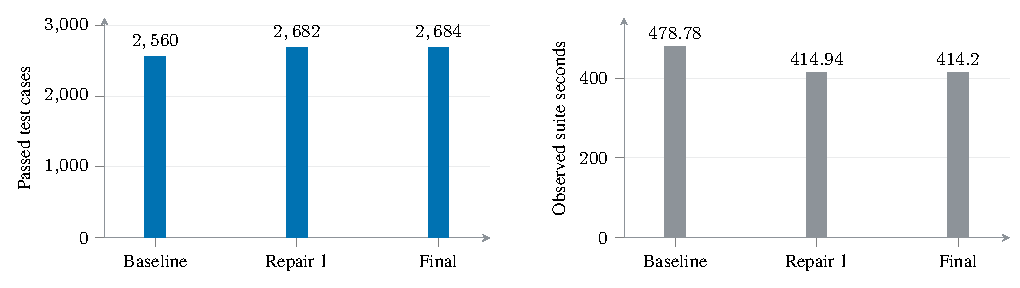
\includegraphics[width=\textwidth]{figures/regression_progress.pdf}
\caption{完整回归的通过数与观测耗时。最终墙钟比初始少 64.58 秒（13.49\%），该差异不能解释为修复带来的因果加速。}\label{fig:regression}
\end{figure}
\source{audit/design_review_20260930/acceptance.json; artifacts/design_review_repair_20260930/final_full_pytest.log}

\subsection{实际 CLI 的状态、分母和证据}
表\ref{tab:cli}逐项报告原验收回执。缺失根和不支持语言在预检阶段阻塞，source\_files=0 表示没有进入有效源码清单统计，不能解释为目标实际有零文件。零候选用例成功完成了一个文件的解析；解析失败用例明确保留一个文件的失败分母。
\begin{table}[htbp]\centering\footnotesize
\begin{tabularx}{\textwidth}{Y L{21mm}c c L{25mm}r}
\toprule 用例 & 运行态 & 源/解析 & 候选/验证/充分 & 性质状态 & 毫秒\\\midrule
\code{literal-mode} & COMPLETED & 1/1 & 1/1/1 & REFUTED & 276.39\\
\code{unknown-mode} & COMPLETED & 1/1 & 1/1/0 & UNKNOWN & 262.45\\
\code{zero-candidates} & COMPLETED & 1/1 & 0/0/0 & -- & 262.43\\
\code{parse-error} & PARTIAL & 1/0 & 0/0/0 & -- & 263.21\\
\code{budget-limited} & PARTIAL & 1/1 & 2/0/0 & UNKNOWN, UNKNOWN & 291.71\\
\code{missing-source} & BLOCKED & 0/0 & 0/0/0 & -- & 256.96\\
\code{unsupported-language} & BLOCKED & 0/0 & 0/0/0 & -- & 272.15\\
\bottomrule\end{tabularx}
\caption{七个真实 CLI 验收用例。每格是单次、自有小源码；0 分母需按预检/清单阶段解释。所有用例均交付 JSON 和 Markdown，模型/目标执行计数均为零。}\label{tab:cli}
\end{table}


\code{literal-mode} 在声明的有界权限位性质上 REFUTED，并不输出全应用 SAFE。\code{unknown-mode} 验证器完成但性质 UNKNOWN，运行仍可 COMPLETED。预算用例含两个候选，在 1800 字节观察上限下两份完整公开证明均未投递：validated=0、sufficient=0、unprocessed=2、公开 observation bytes=0，性质为两个 UNKNOWN。工具调用尝试数为 2，不能写成两次成功验证。其原生产者结果可私有留存，不能用于未交付的强状态。

已有充分证明随后遇到内部失败或取消的保留能力由\emph{另一组}回归验证，该组用例保留先前 REFUTED，停止后续工具并交付局部产物。它不是七个 CLI 中预算用例的结果，两者不能合并叙述。\citep{clireceipt,acceptance}

\begin{figure}[htbp]\centering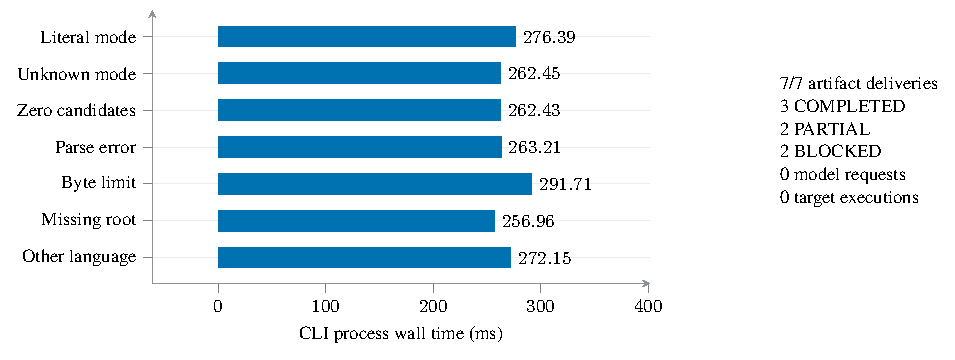
\includegraphics[width=\textwidth]{figures/cli_outcomes.pdf}
\caption{七次真实 console CLI 的运行状态和墙钟。每个用例仅观测一次，极小自有源码且有意包含阻塞与失败路径；不表示真实仓库总体延迟。}\label{fig:cli}
\end{figure}

\subsection{为何必须有多个分母}
这七次运行共有 5 个进入清单的源文件，4 个解析成功、1 个解析失败；发现 4 个候选，2 个验证器完整投递，1 个有充分性质证明，2 个因预算未处理。产物交付 7/7，与性质充分证明 1/4 是不同指标：
\begin{align}
\mathrm{Parsing}_{\mathrm{curated}}&=4/5=80\%,\\
\mathrm{ValidatorCompletion}_{\mathrm{curated}}&=2/4=50\%,\\
\mathrm{SufficientProof}_{\mathrm{curated}}&=1/4=25\%.
\end{align}
候选状态合计 REFUTED 1、UNKNOWN 3，无 SUPPORTED 或 CONFLICT。该计数说明这组路径测试的设计和运行行为，未提供漏洞标签 accuracy、precision、recall 或 FPR。80\%、50\%、25\% 的下降包含有意错误/预算样本，不能据此排列分析器效果优劣。
\begin{figure}[htbp]\centering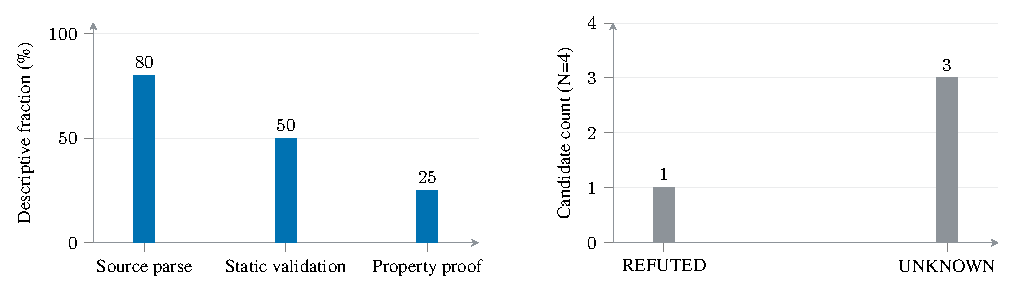
\includegraphics[width=\textwidth]{figures/cli_evidence_denominators.pdf}
\caption{清单、验证完成与充分证明的不同分母，以及四个候选的实际状态。产物成功交付与获得充分性质证明不能互相替代。}
\end{figure}

\subsection{墙钟与成本描述}
七次 console 总墙钟的均值为 \CliMeanMs\ 毫秒，中位数 \CliMedianMs\ 毫秒，范围 \CliMinMs--\CliMaxMs\ 毫秒，样本标准差 \CliStdMs\ 毫秒。每个用例没有重复，未测量并发、冷暖缓存或源码规模曲线，不作生产 SLA 或总体区间推断。内部阶段总计约 11--15 毫秒，与外部 257--292 毫秒不同，主要说明端到端口径包含启动开销；没有单独实验可将差异精确归因到每一模块。

七个用例真实项目模型请求均为 0，physical target executions 均为 0。另一次 transport guard 的 HTTP/socket/live gate 尝试也均为 0。模型费用不应伪造为测量到的 token 单价成本；静态 profile 的 reported\_tokens 未调用 provider，按结果契约保留相应不可用含义。文档写作和内部审阅不纳入项目历史模型实验账本。\citep{transportguard,clireceipt}

\subsection{验收矩阵和门槛状态}
A01--A34 共 34 项，启用静态 profile 的 31 条必需项全通过；A27--A29 是条件 scratch/native 能力，仍未启用/未运行。若将分母写成 34 而宣称全部通过，会掩盖条件范围；若删除三项，又丢失扩展义务。正确当前描述是 \textbf{31/31 必需通过 + 3 条件未提供}。

\begin{figure}[htbp]\centering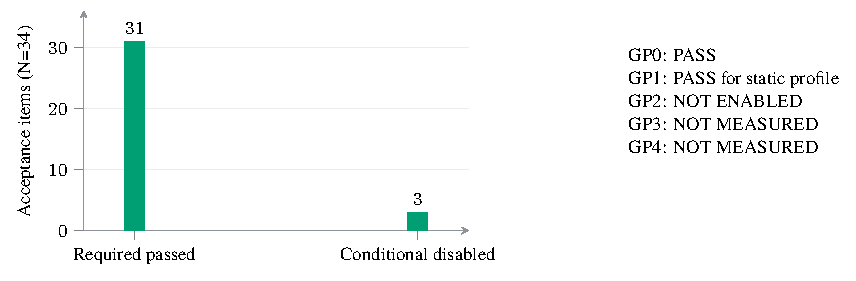
\includegraphics[width=\textwidth]{figures/acceptance_gates.pdf}
\caption{当前验收矩阵与产品门槛。GP0/GP1 通过限于默认静态路径；GP2 未启用，GP3/GP4 尚未测量。附录保留全部 34 项。}\label{fig:acceptance}
\end{figure}

GP0/GP1 只验收离线产物和启用静态控制；GP2 是未启用的条件执行能力。GP3 的人工价值与 GP4 的模型净增量仍未测量，前瞻方案见第\ref{sec:limits}节。

\clearpage
\section{历史研究结果、成本与原 G-A 决策}\label{sec:historical}
\subsection{K1--K4 的工程结果}
\begin{longtable}{L{12mm}L{48mm}L{89mm}}
\caption{截至 2026-09-30 的工程结果与有效解释。}\\
\toprule 工作 & 完成内容 & 有效解释与限制\\\midrule\endfirsthead
\caption[]{（续）}\\
\toprule 工作 & 完成内容 & 有效解释与限制\\\midrule\endhead
K1 & 见证范围与分类前提投递 & 准备与实际执行说明来自测量状态；保留给定场景 a 确认、b 未决控制。\\
K2 & 运行时迁入 \code{runtime/witness/} & 九个迁移模块的 import 归一化文本及 AST 相同；每侧 977 项源码库存、两类 subject 与结果前后相同。\\
K3 & 源码绑定环境从头重建 & 两套 Python 3.12 环境，每侧 141 个依赖版本与 977 项源码绑定一致，未新增读取准入。\\
K4 & E4 共享观察与票数验收 & a 为两张实质票共享一次见证；b 为弃权。E5 用固定票回放，额外实际见证为零。\\
\bottomrule
\end{longtable}

K2 验收中，a 为 \code{CONFIRMED/EXPANDED_OBSERVED}，b 为 \code{UNRESOLVED/LITERAL_OBSERVED}；manifest 唯一变化字段为重建 venv 的 \code{python_executable}。完整 K2 suite 为 2562 passed / 433.32 秒，harness 为 PASS。这些数值属于迁移时的历史验收，不是本次报告重新执行的结果，也不作为新模型进程的 pass stamp。\cite{k2}

这些真实源码 worker 是 developer-scripted 驱动的控制。其工具 provenance 可记录 model-proposed 数据接口，但实验来源仍是给定脚本，不能计为真实模型自主提出成功。

\subsection{M0 与 E-iter 的调用账本}
本节冻结共享授权账本的范围，不包括此前其他实验或文档写作的内部调用。当前工程修复及本报告没有新增项目真实模型 API 请求。

\begin{table}[htbp]
\centering\small
\begin{tabularx}{\textwidth}{L{32mm}r r Y}
\toprule 范围 & 实际请求 & Reported tokens & 观察\\\midrule
M0 阶段 1 & 32 & 191177 & A/B 四格全部弃权；B-a 未完成准备。\\
M0 阶段 2 & 14 & 90153 & 唯一一次 B 两格重跑；实际执行后仍未确认。\\
追加 E-iter & 26 & 166482 & 四格全部弃权，未发生模型驱动的第二场景执行。\\
\midrule
本轮共享账本累计 & 72 & 447812 & 低于 210 请求、2500000 reported tokens 上限。\\
\bottomrule
\end{tabularx}
\caption{统计范围限定为 M0 与追加 E-iter 的共享授权账本。此前历史实验在各自档案中分别保留。}
\end{table}

\begin{table}[htbp]
\centering\small
\begin{tabularx}{\textwidth}{L{37mm}r r L{18mm}Y}
\toprule E-iter 格子 & 请求 & Tokens & 执行次数 & 人工复核的主要缺口\\\midrule
开发见证 a & 6 & 36234 & 1 & F3，场景选择不满足目标见证条件。\\
开发见证 b & 7 & 44985 & 1 & 同一分支与记录前缀缺口；最终弃权。\\
近迁移 callback a & 7 & 45465 & 1 & F4，临时目录不可用，尚未到进程边界。\\
近迁移 callback b & 6 & 39798 & 1 & 同一隔离/临时目录限制。\\
\bottomrule
\end{tabularx}
\caption{E-iter 四格结果。运行标识分别对应 hp003\_a/b 与 hp004\_a/b；后一对为 entry-00390 的近迁移。}
\end{table}

E-iter 的 26 次返回模型 ID 全部为 \code{deepseek-flash}，每次响应具有 usage，原始日志与独立审计一致。真实调用前新进程门禁为 2556 passed / 390.51 秒。每格只有一次物理场景；两份原始 VULNERABLE/UNRESOLVED 提案被准入拒绝，最终四格均 ABSTAIN。固定侧没有 SAFE、producer CONFIRMED 或已准入 VULNERABLE。\cite{eiter}

开发 a/b 场景选择仍落入不同于目标见证的分支，完整紧凑响应已到达模型，后续动作没有形成第二场景尝试。callback 两格在目标候选帧前被隔离环境的临时目录创建阻断，应归因基础设施 F4，不能计成场景选择能力失败或补丁安全。

\begin{figure}[htbp]\centering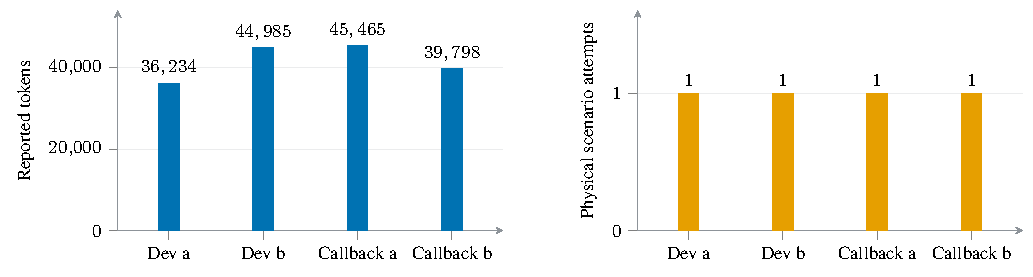
\includegraphics[width=\textwidth]{figures/eiter_cells.pdf}
\caption{E-iter 四格 token 与物理场景次数。每格一个物理场景，四格均 ABSTAIN；配对/同 advisory 数据不构成四个独立仓库样本。}\label{fig:eiter}
\end{figure}

\subsection{失败分类与归因规则}
\begin{table}[htbp]
\centering\small
\begin{tabularx}{\textwidth}{L{11mm}Y}
\toprule 类别 & 预登记解释\\\midrule
F1 & 未调用见证工具，或未走完准备/工具协议。\\
F2 & 场景假设多次被输入 schema 拒绝。\\
F3 & 场景被接受但不足以形成所需见证；必须列出实际缺口。\\
F4 & 见证基础设施、隔离、资源或超时问题。\\
F5 & 见证已确认，但 agent 的最终判定未接纳对应正向证据。\\
F6 & 局部或累计预算耗尽。\\
\bottomrule
\end{tabularx}
\caption{M0 失败分类。自动诊断与人工复核分别保留，类别可以具有伴随因素。}
\end{table}

阶段 1 B-a 的主因是 F1；阶段 2 B-a 主因为 F3，局部 F6 伴随。E-iter 并没有完成模型自主迭代。离线脚本证明工具和原预算可以容纳两个不同场景，不证明真实模型会利用这一能力；提示、协议和投递共同变化的一轮探索也不能隔离预算的因果作用。

\subsection{近迁移、外部样本与 G-A}
3a 的 callback 与原开发样本来自同一 advisory，只是入口近迁移，不是外部项目迁移。离线正确脚本也在临时目录创建处失败，因此 M0 原 3a 的模型运行未满足前置条件；追加 E-iter 包含这两格来自单独授权，不追溯修改原阶段规则。

3b 按预登记顺序冻结前 15 条公告，没有继续从第 16 条挑选。唯一符合源码路径标准的暂定外部候选缺少对应源码版本的目标原生扩展，环境标准未满足，合格外部对数为 0；没有新增 v7、脚本确认或该阶段模型请求。该事实描述当前环境准备能力，没有证明该源码不可构建。

正式 G-A 使用合取条件
\begin{equation}
G\!A=\bigl(\text{原 M0 的 B-a 自主成功}\bigr)
\land\bigl(\text{3b 至少一对外部迁移成功}\bigr).
\end{equation}
两项都不满足，故 G-A = NO。developer-scripted 控制、3a 近迁移和追加 E-iter 不参与救回原门槛。K5--K8 未启动；未使用预算也不构成重新启动这些工作的授权。\cite{gate}


\subsection{其他历史资料的当前解释}
项目还保留 OWASP Java、VulnGym 源码检索、synthetic/V 基线、开发配对完整矩阵与 Jev 分流记录。当前状态页明确将其作为写作时快照，不作为修后源码的成绩。早期部分 fixture 曾将权限模式误声明为竞态、将源码字符串形状作为授权证明，或依赖 expected-role 过滤；仅凭旧标签计分无法满足现行性质与范围契约。本文没有重审这些整批请求，不把旧正确率并入当前结果，也不把 72 请求写成项目从创建以来的总用量。\citep{status,contract}

\subsection{历史成本的描述性分析}
三个阶段的请求和 token 分别占总量的不同份额。M0 阶段 1 使用 32/72 请求（44.44\%）和 191177/447812 tokens（42.69\%）；阶段 2 为 14/72（19.44\%）和 90153/447812（20.13\%）；E-iter 为 26/72（36.11\%）和 166482/447812（37.18\%）。这是投入分配，不是各阶段的信息价值测量。

\begin{figure}[htbp]\centering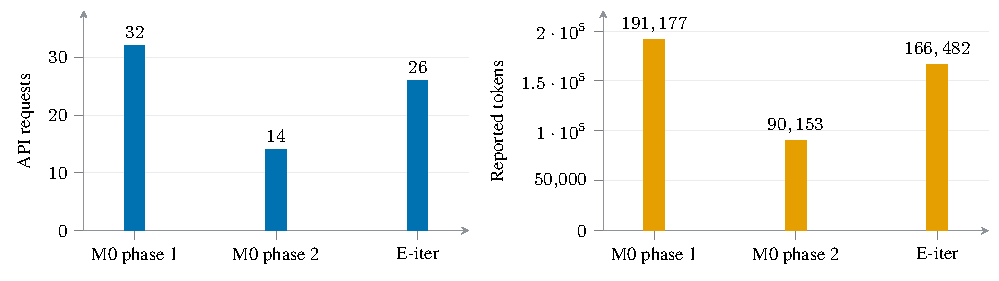
\includegraphics[width=\textwidth]{figures/historical_usage.pdf}
\caption{共享历史账本分阶段用量。Reported tokens 是 provider 响应中的计数，与观察字节预算分开；请求响应解析失败也应保留用量。}\label{fig:usage}
\end{figure}

平均每个实际请求为 \AvgTokensPerRequest\ reported tokens，混合 planner、循环、输入和输出，不能当作一次固定任务的标准成本。E-iter 四格 tokens 均值 41620.5，范围 36234--45465，样本标准差 4413.46；最大/最小约 1.25。这四格每格均一次物理场景，显示 token 数与场景尝试数不是同一个量。相同或更高 token 投入并没有在本轮产生自主确认，但没有匹配对照可估计 token 增量的因果效果。

\begin{figure}[htbp]\centering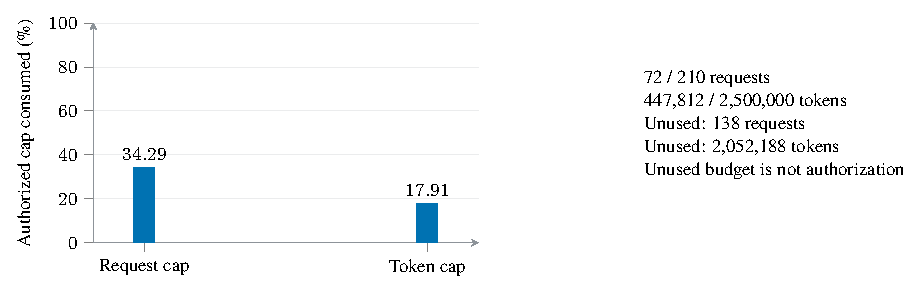
\includegraphics[width=\textwidth]{figures/budget_utilization.pdf}
\caption{历史授权上限的使用比例。请求使用 34.29\%，tokens 使用 17.91\%；余额只是旧账本数值，不授权新实验。}
\end{figure}

余下 138 请求与 2052188 tokens 不改变 G-A，也不等于当前可以再次调用。所有返回模型 ID 以原始响应为准，未知 usage 不能补为零。未提供完整历史价格配置和账单，本文不将 reported tokens 换算成货币费用。

\section{当前定位、限制与前瞻评价}
\label{sec:limits}
\subsection{已经建立的结论}
项目已经有可独立运行的离线 Python 静态审查交付路径：使用者明确选择源码根，系统保留字节身份、解析分母、候选、已登记事实、有限性质状态、缺项和一致产物。共享内核能够拒绝已知的错 subject、弱静态确认、晚到同范围冲突和嵌套别名漂移。保留研究系统可以组织有界检索、规划、类型化工具、有限 ReAct、单专家票、quorum 与条件执行见证。

在少量已选开发候选和给定分类场景中，见证仍定位为\textbf{有界确认工具}。其正向控制和 K2 迁移等价性已经建立；自主场景提出、合格外部迁移、公开入口以及 fresh held-out 泛化没有由当前证据建立。原 G-A=NO 与新产品 GP0/GP1 的工程通过能够同时成立，回答的是不同问题。

\begin{longtable}{L{33mm}L{70mm}L{46mm}}
\caption{当前边界、已观察影响和下一步证据要求。}\\
\toprule 边界 & 当前证据 & 需要补的证据\\\midrule\endfirsthead
\caption[]{（续）}\\
\toprule 边界 & 当前证据 & 需要补的证据\\\midrule\endhead
静态语义 & 未支持 helper、动态分派、外部库及对象协议保持 UNKNOWN；有限模型有正例 & 对明确语义逐项新增正反控制，不宣称整个 Python 完备。\\
性质与全应用 & 有界 REFUTED/SUPPORTED 明确不覆盖应用安全 & 另行定义资产、路径、输入域和安全性质。\\
源码与环境 & 产品身份覆盖所选 Python 清单；静态 execution digest 为 null & 条件执行需可信环境清单和单独准入。\\
场景选择 & E-iter 四格没有第二物理场景；两格因分支，两格因环境 & 独立冻结场景研究、反馈、重复次数和预算。\\
公开入口 & callback 直接调用没有公开 parser；本地调用不建立远程权限 & 显式入口/部署范围及授权依据。\\
文件系统写入 & 历史隔离阻止临时目录，sink 尚未到达 & T10 私有 scratch 的拥有者夹具和写入边界控制。\\
原生扩展 & 3b 暂定外部候选未完成对应环境准备 & T11 可信源码、工具链、hash 和可复核构建。\\
多专家与早停 & 可共享一份原观察；固定已知票保证有限 & 独立 live 增量与成本实验；未知未来证据仍是边界。\\
数据盲性 & 开发、oracle 和暴露元数据不具 held-out 资格 & 新鲜、事前冻结、标签隔离且按仓库计分。\\
用户价值 & GP3/GP4 尚未测量 & 配对人工审查与可选模型说明的净增量。\\
\bottomrule\end{longtable}

\subsection{工程数值能说明什么}
2684 个通过用例说明当前声明控制没有在完整套件中失败；它不枚举所有程序输入，也不是 detector benchmark。31 条必需验收证明静态交付契约，未覆盖三个条件能力。七个 CLI 产物用例证明不同运行状态下可交付，并显示约 269 毫秒的小用例启动墙钟；无法外推大仓库吞吐。

历史 447812 tokens 的投入以及四格 ABSTAIN 说明本轮自主任务没有达到门槛；不能在缺少反事实对照时将原因唯一归为模型、预算或协议。F3 与 F4 的区分使后续研究能针对场景/环境分别设计验证。0 合格外部样本的含义是当前准入管线没有完成迁移测量，而不是估计某总体成功率为零。

\subsection{已冻结但未执行的增量评估协议}
T14 前瞻方案以仓库为统计单位，纳入新鲜项目拥有或明确授权源码，按语言、性质、源码规模和初始上下文缺口分层；排除 oracle、开发专用、已暴露 held-out 和未授权材料。源码、性质契约、基线事实与准入上下文事前冻结，评价标签不进入 detector prompts、路径别名或源码选择。\citep{increment}

配对臂为原人工流程、离线产品报告和条件模型说明。前两者项目模型请求为零；模型说明仍关闭，未设新请求或 token 授权。说明只能引用合法事实与缺项，不能修改性质状态。审阅顺序在审阅者间平衡，保留排除和失败项，记录人工秒数、事实错误、缺项识别、行动性、全部模型请求/usage、unknown usage 与端到端墙钟。

\begin{pseudocode}{alg:future}{尚未执行的前瞻 paired-review 协议}
\Pinput{事前冻结且明确授权的新鲜仓库、独立评价记录、reviewer 与预算}
\Poutput{仓库级配对质量/时间差及完整成本；允许无收益结果}
\Pstep{核对数据角色、授权、源码和契约身份；泄漏或漂移立即停止。}
\Pstep{先冻结同一基线事实和上下文，再运行原人工流程与离线产品报告臂。}
\Pstep{平衡 reviewer 的臂顺序，记录时间、事实错误、正确缺项及行动价值。}
\Pstep{仅在单独授权后启用模型说明；不允许说明改写性质状态。}
\Pstep{以仓库为单位汇总配对差，保留未完成/未知项及所有成本。}
\Pstep{按事前分析规则判断 GP3/GP4；无净收益同样为有效结果。}
\end{pseudocode}

若之后设计区间分析，应事前确定以仓库为单元的配对 bootstrap 或其他适用方法、样本量和缺失处理。当前冻结协议只确立仓库级配对汇总与完整记账，没有事后假装已完成显著性实验。planner、Jev、多专家或 target execution 进入产品需要独立可复现净收益，不能因为组件已存在就自动启用。

\subsection{延后路线和发布状态}
T10/T11 的条件能力未启用，T14 只有协议。历史 K5--K8 没有启动。定位报告列出的四条路线仍分别是私有临时目录、原生扩展源码构建、场景提出研究和新评测集；这些路线的设计依赖继续保留，启用时需选择具体范围并重新预登记。\citep{positioning,architectureplan}

当前修复已验收但尚未提交，HEAD 没有因这些修复产生新提交；工作区也不是 clean。报告属于工作树快照，源码聚合 SHA-256 与输入回执哈希用于复核。历史汇总 JSON 已修正 K2、G-A 和统计来源，旧值只保留在历史快照对象。没有借重写历史或追加模型实验改善本报告结论。

\section{复现、产物目录与事实更新}
\subsection{可直接复用的默认产品入口}
在项目 uv 环境中，\code{doctor} 给出能力与输入诊断，\code{review} 生成离线结果。选择拥有或明确授权的本地 Python 源码，输出目录应尚不存在：
\begin{lstlisting}[language=bash,caption={默认静态产品入口；路径由使用者明确选择。}]
uv run --no-sync cv-agent doctor /path/to/authorized/source
uv run --no-sync cv-agent review /path/to/authorized/source \
  --output /path/to/new-review-run
\end{lstlisting}
默认观察预算 8192 bytes，可显式设置；初始范围与扩展通过 grants 文件声明，字段见附录。命令没有默认目标执行或真实模型调用。真实模型研究入口仍遵守完整 pytest gate、独立实验授权、请求账本和数据角色。

\subsection{本报告的构建}
源码包包括 \code{main.tex}、分节正文、\code{references.bib}、规范数据、矢量图的 PDF/PGFPlots 源码及构建脚本。字体使用已安装的 Source Han Serif SC、Noto Sans SC 和 TeX Gyre；伪代码框由 tcolorbox 编排。图中数值来自冻结回执，不从截图读数。引用的 OneReason 只提供单栏技术报告版式参考。\citep{onereason}

\begin{lstlisting}[language=bash,caption={从项目根目录编译；不安装依赖、不开启 shell escape。}]
python3 docs/reports/cv_agent_technical_report_2026-10-01/scripts/build.py
# Optional: regenerate only vector charts from the frozen report_data.json
python3 docs/reports/cv_agent_technical_report_2026-10-01/scripts/plot_figures.py
\end{lstlisting}
构建运行 XeLaTeX、BibTeX 和稳定交叉引用所需重复编译。不会运行检测器、模型或 witness。重新收集项目数据是独立离线操作，\code{scripts/collect_data.py} 从既有回执及当前源码统计生成数据，测试用例数读取已归档的 collect-only 日志；它不自动替换报告结论或重跑历史模型实验。

\subsection{来源与复核文件}
\begin{longtable}{L{76mm}L{73mm}}
\caption{报告事实的主要来源；路径相对项目根。已收集输入与逐 CLI 结果的 SHA-256 在 data/report\_data.json，文档产物哈希另记于构建回执。}\\
\toprule 文件或目录 & 用途\\\midrule\endfirsthead
\caption[]{（续）}\\
\toprule 文件或目录 & 用途\\\midrule\endhead
\code{audit/design_review_20260930/baseline.json} & 核查基线、初始失败与已有文件保护。\\
\code{audit/design_review_20260930/verification.md} & 已复现问题、正反控制、边界和失败解释。\\
\code{audit/design_review_20260930/tasks.json} & T00--T14 实际文件、命令和前后日志。\\
\code{audit/design_review_20260930/acceptance.json} & 完整套件、harness、34 项验收及 GP 状态。\\
\code{audit/design_review_20260930/cli-acceptance.json} & 七个实际 console 用例的状态、计数与墙钟。\\
\code{audit/design_review_20260930/transport-guard.json} & HTTP/socket/live gate 的拒绝式零尝试控制。\\
\code{audit/design_review_20260930/final-source-manifest.json} & 修复工作树源码清单。\\
\code{.hermes/plans/2026-09-30-E-iter-results.json} & 四格请求、token、物理场景与失败归因。\\
\code{.hermes/plans/2026-09-30-G-A-decision.json} & 原门槛的正式 NO 和不计入救回的范围。\\
\code{.hermes/plans/2026-09-30-remaining-work-final-summary.json} & K2、历史分阶段账本和来源修正。\\
\code{.hermes/plans/2026-09-30-product-increment-preregistration.json} & 尚未执行的 GP3/GP4 前瞻协议。\\
\code{docs/reports/cv_agent_technical_report_2026-10-01/data/report_data.json} & 本文数字、聚合源码摘要与输入文件哈希。\\
\code{artifacts/technical_report_20261001/build_receipt.json} & 本报告源码/PDF 哈希、结构与编译/视觉验证。\\
\bottomrule\end{longtable}

\subsection{文档复核与更新纪律}
LaTeX 编译、数值核对和 PDF 渲染审查验证这份文档能被阅读与追溯，不是模型实验准入回执。完整测试 2684 passed 属于本次报告引用的已归档最终修复源码，报告工作不修改分析源代码，也不使用历史 pass stamp 发出请求。

本轮检索并下载公开版式参考；项目层面没有新增模型 API 实验、目标执行或安装。旧报告与审查 PDF 原样保留。后续更新保留原请求、失败日志、来源披露和门槛决策。

\clearpage
\appendix
\section{产品接口、字段与状态速查}
\subsection{命令行参数}
\begin{longtable}{L{42mm}L{24mm}L{83mm}}
\caption{当前产品 CLI 参数。研究命令沿用独立协议，不在此扩张实验授权。}\\
\toprule 参数 & 默认 / 要求 & 含义\\\midrule\endfirsthead
\caption[]{（续）}\\
\toprule 参数 & 默认 / 要求 & 含义\\\midrule\endhead
\cmd{review source_root} & 必需 & 明确选择的本地授权源码根。\\
\code{--output} & 必需 & 新目录；已存在则拒绝覆盖。\\
\code{--language} & python & 默认产品只提供 Python；其他语言阻塞。\\
\code{--observation-bytes} & 8192 & 完整工具观察公共投递池，单位 bytes。\\
\code{--context-grants} & 无 & 显式 source-grants-v1 manifest。\\
\code{--context-bytes} & 8192 & 上下文扩展的完整封装预算。\\
\cmd{doctor source_root} & 必需 & 预检能力和输入，输出 JSON。\\
\cmd{doctor --language} & python & 预检的语言。\\
\cmd{doctor --property-id} & 可选 & 预检声明的性质；不推导标签。\\
\bottomrule\end{longtable}
\code{review} 仅在 COMPLETED 时返回 0，其他运行态返回 2；\code{doctor} ready 返回 0，非 ready 返回 2。参数语法错误由 argparse 明确处理。harness-check 和 readiness 是研究契约/产物诊断，不能当作 review 的模型旁路。

\subsection{显式 grant manifest}
以下使用中性路径和解释理由，仅描述接口，不包含漏洞输入：
\begin{lstlisting}[caption={source-grants-v1 的初始范围与显式扩展。}]
{
  "version": "source-grants-v1",
  "initial": [
    {"path": "entry.py", "start_line": 1, "end_line": 4,
     "reason": "selected entry"}
  ],
  "extensions": [
    {"path": "helper.py", "start_line": 1, "end_line": 2,
     "reason": "explicit helper context"}
  ]
}
\end{lstlisting}
start/end 是包含端点的正整数。规范路径必须属于授权清单；后续扩展重读字节并核对摘要。每条准入回执包含 admission ID、路径、行号、reason、ADMITTED/REJECTED、reason code 和 delivered bytes。文件名可见不表示该文件其他 span 已准入。

\Needspace{14\baselineskip}
\subsection{ReviewResult 字段}
\begin{longtable}{L{45mm}L{104mm}}
\caption{公共结果的顶层字段与约束。}\\
\toprule 字段 & 内容和约束\\\midrule\endfirsthead
\caption[]{（续）}\\
\toprule 字段 & 内容和约束\\\midrule\endhead
\code{schema_version} & product-review-v1；非法版本拒绝。\\
\code{profile_id} & product\_triage\_v1；不伪装为研究 E 系统。\\
\code{run_id/run_state} & 独立运行标识和五种运行态。\\
\code{identity} & product-identity-v1；源码/分析/视图摘要与可选执行摘要。\\
\code{findings} & 候选、subject、性质契约、四值状态、事实、缺项、下一步及证据引用。\\
\code{evidence_receipts} & 原生产者、工具、原验证状态、独立静态投影、方法、范围、投递、内容哈希及产品身份。\\
\code{capabilities} & 语言、性质、方法、AVAILABLE/UNSUPPORTED/BLOCKED、required、reason 和检查版本。\\
\code{diagnoses} & 阶段、原因码、消息、责任方、重试政策、必需输入、影响候选及私有日志引用。\\
\code{scope_admissions} & 每条准入或拒绝的行范围、理由和 bytes。\\
\code{counts} & 源清单、解析、候选、验证完成、充分证据、未处理、索引及准入文档的独立分母。\\
\code{accounting} & 模型请求固定 0；工具/物理执行、观察/context bytes、分阶段耗时与可用 token 字段。\\
\code{artifacts} & 同一次运行的 JSON、Markdown、私有观察等引用。\\
\bottomrule\end{longtable}

\subsection{回执与诊断的最小解释}
\code{EvidenceReceipt} 中 \code{observation_id} 是公开引用，\code{producer_id} 是调用身份，\code{content_sha256} 对应原始内容。\code{method_version=tool-contract-v1} 约束方法，\code{coverage=candidate/local} 约束范围。\code{delivered} 不等于执行发生；\code{validation_status} 不等于产品性质状态；\code{accepted_static_status} 只适配注册命令静态逻辑。proof 必须再次通过同 subject、合法方法和完整投递检查。

诊断 stage 取 input、preflight、index、analysis、validation、reduction、presentation 或 runtime；owner 为 user、environment、runtime 或 analyzer；retry policy 为 never、after\_input、after\_environment\_change 或 manual。历史 F1--F6 映射字段可空，不强迫每个产品故障归入模型场景失败。公共诊断保持缺项可行动，内部 traceback 留在私有产物。

\subsection{语义与操作不变量}
\begin{enumerate}
\item candidate、subject、性质契约、产品 source 和 analysis 身份一致；纯展示别名不增加权威。
\item 完整投递、充分范围和合法证明方法是强状态的必要条件；UNKNOWN 不抹去已有充分 proof。
\item 同身份同完整范围正反 proof 都存在时只能 CONFLICT；局部事实不升级。
\item parsed + parse\_errors 不超过 source\_files；候选数与 findings 数相等；充分证据数与非 UNKNOWN finding 数一致。
\item COMPLETED 不允许隐藏解析失败、未处理候选或不可用必需能力；可完整完成一个仍为 UNKNOWN 的验证。
\item 模型、目标执行、planner、Jev 和早停不属于默认产品；可选能力缺失不阻塞独立静态任务。
\item 预算投递和上下文扩展先计费成功后更新权威视图；缓存不隐式再执行。
\item application\_security=NOT\_ASSESSED，remote/public 标志为 false；任何 finding 不证明整个应用安全。
\end{enumerate}

\section{逐项任务与完整验收矩阵}
\subsection{实施任务 T00--T14}
本附录编号来自本次设计核查任务卡，与测试契约 T01--T16 不同。任务 T00--T09、T12、T13 已按默认静态 profile 完成；T10/T11 为条件能力；T14 仅完成前瞻协议。
\begin{longtable}{L{14mm}L{69mm}L{66mm}}
\caption{任务完成范围；不将条件项或协议冻结视为测量完成。}\\
\toprule 任务 & 内容 & 当前状态\\\midrule\endfirsthead
\caption[]{（续）}\\
\toprule 任务 & 内容 & 当前状态\\\midrule\endhead
T00 & 实际基线、旧修改/历史保护、特征化 & 默认静态范围完成。\\
T01 & 性质契约、状态/身份/分母与导出 schema & 默认静态范围完成。\\
T02 & 产品能力预检与功能检查注册 & 默认静态范围完成。\\
T03 & 独立产品服务和真实 CLI & 默认静态范围完成。\\
T04 & 结构化诊断、准备/等待输入和补项 & 默认静态范围完成。\\
T05 & 公共快照与分层身份 & 默认静态范围完成；私有反射非保证。\\
T06 & 全局证据归并与研究重新准入 & 已知投递事实范围完成。\\
T07 & 真实数据依赖、有限控制与图上限 & 默认静态范围完成，旧研究义务保留。\\
T08 & 守恒证书池、缓存及独立投递计费 & 默认静态范围完成；服务无必成证明预留。\\
T09 & 显式行范围视图与付费扩展 & 默认静态范围完成。\\
T10 & 私有 scratch 与生命周期 & 条件未启用。\\
T11 & 可信 native build & 条件未启用。\\
T12 & runtime 记账、只读恢复与取消/脱敏 & 启用静态范围及保留控制完成。\\
T13 & 完整 pytest、harness、真实 CLI 与矩阵 & 默认静态范围已验收。\\
T14 & 人工/模型增量协议 & 协议冻结；GP3/GP4 未测量。\\
\bottomrule\end{longtable}

\subsection{A01--A34 的验收}
\begin{longtable}{L{11mm}L{11mm}L{97mm}L{30mm}}
\caption{全部 34 个验收项。31 必需项通过，3 条件项保留未提供。每项测试路径和日志 SHA-256 在 acceptance.json/tasks.json。}\\
\toprule 项 & 任务 & 验证行为 & 结果\\\midrule\endfirsthead
\caption[]{（续）}\\
\toprule 项 & 任务 & 验证行为 & 结果\\\midrule\endhead
A01 & T00 & 实际基线、历史保护、完整套件与特征化 & 通过\\
A02 & T01 & 20 个运行/性质组合、非法状态和计数 & 通过\\
A03 & T01 & 精确 subject、性质、行、source/analysis 绑定 & 通过\\
A04 & T01 & 应用未评估和 remote/public false & 通过\\
A05 & T02 & 无 provider/witness 的静态能力 & 通过\\
A06 & T02 & 已注册自有检查缺依赖及显式恢复 & 通过\\
A07 & T03 & 实际 console 与 HTTP/socket/gate 拒绝 spy & 通过\\
A08 & T03 & 零候选与解析失败分母/产物 & 通过\\
A09 & T03 & 内部失败保留既有 proof 和局部产物 & 通过\\
A10 & T04 & F4 环境与 F1 准备区分，F1--F6 保留 & 通过\\
A11 & T04 & 等待输入、补项及依赖恢复，准备非完成 & 通过\\
A12 & T05 & 五项嵌套别名回归及源码正反控制 & 通过\\
A13 & T05 & 源码/helper/import/环境漂移与视图分离 & 通过\\
A14 & T08 & 别名与两个原 ID 区分，保留验证记账 & 通过\\
A15 & T06 & 晚到冲突两种顺序，slow/fast 重新准入 & 通过\\
A16 & T06 & 局部反事实不抹去完整独立支持 & 通过\\
A17 & T06 & 三个引用别名不增加强度 & 通过\\
A18 & T06 & UNKNOWN 不抹证明，helper 引用保留 & 通过\\
A19 & T07 & 不可用可选任务与独立静态任务，真实依赖阻塞 & 通过\\
A20 & T07 & 完成 UNRESOLVED 解锁，准备/error 不解锁 & 通过\\
A21 & T07 & 固定无效动作限额及无进展图终止 & 通过\\
A22 & T08 & 2500+1000+1000+1000 完整证书在 8192 内 & 通过\\
A23 & T08 & JSON 外壳/ID 计费，裁剪及局部错误不证明 & 通过\\
A24 & T08 & 缓存投递计 bytes，原执行唯一且保护预留 & 通过\\
A25 & T09 & 授权 helper 投递计费；失败扩展不准入 & 通过\\
A26 & T09 & 同路径不准入其他行范围，旧 E 预算保留 & 通过\\
A27 & T10 & 私有 scratch 能力未启用 & 未启用 / 未运行\\
A28 & T10 & 新 scratch 生命周期未启用，保留旧只读控制 & 未启用 / 未运行\\
A29 & T11 & 可信 native build 未启用 & 未启用 / 未运行\\
A30 & T12 & 每进程完整 gate、漂移及失败拒绝 & 通过\\
A31 & T07 & 八个实际任务，循环受图上限 16 约束 & 通过\\
A32 & T12 & 六个最后名额竞争者及畸形内容 usage 保留 & 通过\\
A33 & T12 & 半写 journal、未知 reservation、取消无后续调用 & 通过\\
A34 & T12 & 伪状态/源码 key 留数据私有，transport key 脱敏 & 通过\\
\bottomrule\end{longtable}
\source{audit/design_review_20260930/acceptance.json; audit/design_review_20260930/tasks.json}
\subsection{完整日志与源码摘要}
最终完整日志 SHA-256 为 \code{d3a2bc10a5e0d9480039c18486c74689d8a3970fa20a19ab4af445c7efd1c341}。报告收集的 230 个 Python 源文件聚合摘要为 \code{c1bd6bb77ff68a2449b6b7d8af33814e286c224fd733e960f7b0e5ac89b58fa8}；算法按排序路径加入路径 bytes、分隔零字节和每文件 SHA-256 bytes。该摘要用于报告工作树复核，与产品 source-bytes-v1 或研究 ValidationSubject 的摘要算法不同。

\subsection{保留的语义测试契约}
C1--C6 是源码语义的规范职责。下表来自当前测试契约；T01--T16 是语义回归编号，与上文实施任务卡不同。
\begin{longtable}{L{13mm}L{35mm}L{101mm}}
\caption{语义契约及其执行要求。}\\
\toprule 契约 & 主题 & 核心要求\\\midrule\endfirsthead
\caption[]{（续）}\\
\toprule 契约 & 主题 & 核心要求\\\midrule\endhead
C1 & 判断对象 & 候选、源码、位置、性质、范围及前提完整绑定；局部事实不升级为不匹配性质的证明。\\
C2 & 值与执行效果 & 区分已知值、来源、未知值，正常继续、终止、异常，及相关副作用与覆盖缺口。\\
C3 & 求值顺序与摘要 & 短路、条件表达式、调用实参与 helper 服从同一副作用规则；摘要需要身份和输入前提。\\
C4 & 路径合并 & 完整危险路径、全范围安全、未解析路径、同范围冲突分别处理；重复条件关联不能制造假路径。\\
C5 & 证据准入 & 全部相关观察约束判决；调用顺序、引用角色和静态扫描增删不能替代语义事实。\\
C6 & 收尾与依赖 & 终止不降低证据门槛；任务结束不自动等于验证完成；非法协议不伪装成普通弃权。\\
\bottomrule
\end{longtable}
\begin{longtable}{L{13mm}L{46mm}L{90mm}}
\caption{测试契约要求的验收类别。当前主链核验不表示所有组合已穷尽。\citep{contract}}\label{tab:acceptance}\\
\toprule 类别 & 检查主题 & 关键行为与正控制\\\midrule\endfirsthead
\caption[]{（续）}\\
\toprule 类别 & 检查主题 & 关键行为与正控制\\\midrule\endhead
T01 & caller/helper 范围 & 不借 helper 局部安全抵消 caller 危险；双方受支持安全时仍保留安全判断。\\
T02 & 位置与切片 & 不同 sink、偏移、装饰器及 helper 不错借身份；准确位置正例可通过。\\
T03 & 表达式副作用 & 条件、短路、比较、海象和参数位置的相关操作被保留或明确未解析。\\
T04 & 纯度与死分支 & 确定死分支和未调用延迟体不虚构执行；未知对象协议不默认纯净。\\
T05 & helper 执行效果 & 参数、别名、全局和函数重绑定缺口不被未使用返回值抹去；独立完整危险事实保留。\\
T06 & 解包与终止 & 全成功、全失败、成功与失败/未知组合、嵌套及异常边界保持正确后继。\\
T07 & 输入来源 & 未知值不等于已证明输入；错来源不套用摘要；具体前提保持正例。\\
T08 & 消费上下文 & 正常保护、后续拼接、二次解释与非 shell 消费区别处理。\\
T09 & 条件关联 & 相同条件重复检查不生成不可能路径；绑定改变和未声明平台保持缺口。\\
T10 & 权限覆盖 & 不同目标和时间顺序不抵消；位模式证明不升级为竞态证明。\\
T11 & 引用与取证不变性 & 角色、省略、静态扫描和独立读取顺序不能改变同一语义事实的约束。\\
T12 & 路径和证明冲突 & 不同独立路径与同范围互斥证明分别处理；真实危险路径正例仍可用。\\
T13 & 身份与投递 & 完整且匹配的证明可用；错 subject、性质、摘要、引用及裁剪/抑制/错误被拒。\\
T14 & 收尾和用量 & 普通与末步阶段同一证据门槛，零尝试不伪造成票，全部实际请求记账。\\
T15 & 验证完成与依赖 & 未完成必需验证器阻塞直接和传递依赖；已完成未决与未完成分别记录。\\
T16 & 多任务与 quorum & 同一专家一票，弱票不能凑证明，固定票早停与全量标签一致。\\
\bottomrule
\end{longtable}

\section{核心模块阅读索引}
表中路径以 \code{src/cv_agent/} 为基准；同一行的短文件名或子目录沿用首项显示的所属包。
\begin{longtable}{L{66mm}L{83mm}}
\caption{源码定位与理解顺序。所有路径均以 \code{src/cv_agent/} 为前缀。}\\
\toprule 位置 & 应阅读的逻辑\\\midrule\endfirsthead
\caption[]{（续）}\\
\toprule 位置 & 应阅读的逻辑\\\midrule\endhead
\code{domain/types.py}, \code{evidence.py}, \code{review.py}, \code{chat.py} & 候选、subject、观察、任务与票，以及 provider-neutral 消息和 usage。\\
\code{domain/validation_protocol.py} & 准备状态、缺字段 destination、dataset/model 模式及继续动作。\\
\code{code_adapters/python.py}, \code{java.py}, \code{javascript.py}, \code{go.py} & 多语言切片、定义、调用与元数据的生成。\\
\code{code_adapters/source_files.py}, \code{fallback.py}, \code{repository.py} & 安全读取、fallback 层级及仓库文档组装。\\
\code{agents/discovery.py}, \code{scanner.py} & 标签无关的 Python 源码清单与有限候选规则。\\
\code{retrieval/index.py}, \code{context.py}, \code{dependencies.py}, \code{tokens.py} & 图绑定、文本/图/hybrid 排序、局部窗口、预算和序列化拟合。\\
\code{retrieval/bm25.py} & 独立 BM25 元数据诊断。\\
\code{agents/workflow.py} & LangGraph 状态、依赖调度、累积票与最终结果。\\
\code{agents/planning.py}, \code{plan_policy.py} & 计划提示、schema、必要任务与政策组合。\\
\code{agents/react.py} & 模型/工具循环、纠正、final-only 阶段及用量累计。\\
\code{agents/evidence_policy.py} & 性质与范围准入、相关反证、冲突、投递及必需验证完成。\\
\code{agents/routing.py}, \code{applicability.py} & 可选 Jev 分流及独立专家适用性政策。\\
\code{agents/voting.py}, \code{validator_accounting.py} & 单票/quorum、早停与原始观察共享计数。\\
\code{tools/registry.py}, \code{repository.py}, \code{identity.py} & 工具 schema 与作用域、源码查询、重复记忆及 subject 构造。\\
\code{tools/analysis/commands.py}, \code{python_flow.py}, \code{python_probe.py} & 有界命令、数据流和 AST 输入探针。\\
\code{tools/validation/permissions.py}, \code{authorization.py}, \code{commands.py} & 对应性质的观察封装与语义边界。\\
\code{tools/validation/fixtures.py}, \code{comparison.py} & 注册夹具、loopback 案例与源码差分。\\
\code{tools/validation/bounded_witness.py}, \code{witness_manifest.py}, \code{witness_scenario.py}, \code{witness_response.py} & 见证服务、系统清单、分类场景和 compact 投递。\\
\code{runtime/witness/kernel.py}, \code{contract.py}, \code{scenario_runtime.py} & 源码绑定 worker、正向 proof contract 与场景执行。\\
\code{runtime/witness/obligations/values.py}, \code{branches.py}, \code{preexec.py} & 真实值、分支和 preexec 义务。\\
\code{runtime/witness/accounting.py}, \code{tracer.py}, \code{isolation_policy.py} & 执行资源、读取追踪与身份绑定准入。\\
\code{runtime/model.py}, \code{provider.py}, \code{admission.py}, \code{jev.py} & 传输、provider 组装、完整 pytest 门禁和 choice 协议。\\
\code{runtime/budget.py}, \code{journal.py}, \code{snapshots.py}, \code{provenance.py} & 预算、耐久事件、源码快照及 Git 身份。\\
\code{harness/models.py}, \code{defaults.py}, \code{validation.py} & 不可变实验声明、E/V 默认系统和约束核对。\\
\code{evaluation/execution.py}, \code{lifecycle.py}, \code{results.py}, \code{metrics.py} & 候选执行、实验组织、输出、三值指标和配对比较。\\
\code{evaluation/datasets/}, \code{protocols/}, \code{discovery.py} & 数据角色、输入/标签分离、专项验收与发现计分。\\
\code{evaluation/preparation/prepare_witness_environment.py}, \code{witness_import_worker.py}, \code{witness_metadata.py} & 锁定环境、metadata-only 目标安装、受限导入与上下文产物。\\
\code{evaluation/runners/}, \code{diagnostics/} & 显式实验入口、审计、预检和已完成运行复核；不能仅凭名字认定调用离线。\\
\code{baselines/}, \code{cli.py} & 确定性历史对照与命令派发。\\
\code{application/preflight.py}, \code{service.py}, \code{diagnostics.py} & 独立产品能力声明、分析编排和结构化诊断。\\
\code{application/identity.py}, \code{context.py} & 字节与分析身份、行区间准入及事务性扩展。\\
\code{application/evidence.py}, \code{delivery.py}, \code{controller.py} & 全局归并、完整证书预算与独立任务控制。\\
\code{domain/product_result.py}, \code{presentation/report.py} & 版本化结果契约和只读渲染。\\
\code{runtime/redaction.py}, \code{journal.py::audit_journal} & 展示脱敏、已知密钥保护与保守只读恢复审计。\\
\bottomrule
\end{longtable}

\section{工具目录与输出解释}
\begin{longtable}{L{61mm}L{88mm}}
\caption{当前注册工具族。工具是否可用及可支持的证明状态由本次运行的能力声明决定。}\\
\toprule 工具 & 职责和主要限制\\\midrule\endfirsthead
\caption[]{（续）}\\
\toprule 工具 & 职责和主要限制\\\midrule\endhead
\code{search_symbols} & 在准入文档中搜索符号，不扩展检索路径。\\
\code{read_span} & 读取已准入切片或范围，完整响应按序列化预算计数。\\
\code{get_callers}, \code{get_callees} & 提供已建立图边与有限邻居，图事实不直接证明动态可达。\\
\code{find_references} & 在准入源码中查找引用，保留缺失和绑定限制。\\
\code{run_static_check} & 发现有限模式与操作类型，保持静态观察范围。\\
\code{find_sources}, \code{find_sinks}, \code{find_sanitizers} & 定位来源、消费和处理候选；存在名称不是完整证明。\\
\code{trace_dataflow} & 有界 may-flow、参数绑定和缺边记录；保持 UNRESOLVED。\\
\code{inspect_command_construction} & 命令来源、转换、路径、消费上下文和执行效果检查。\\
\code{probe_python_eval} & 有界 AST 输入控制探针，匹配动态求值性质。\\
\code{validate_permission_mode} & 特定权限 mode 性质的静态验证，不能证明目录竞态。\\
\code{get_routes}, \code{get_guards} & 路由与守卫事实；没有匹配不表示绕过成立。\\
\code{inspect_principal}, \code{inspect_resource_scope} & 主体及对象/租户范围的有界提取。\\
\code{compare_route_and_service_guard} & 已准入路由及服务调用链的守卫对照。\\
\code{run_fixture_test} & 运行注册项目夹具，必须匹配 subject、性质和充分 proof scope。\\
\code{run_loopback_http_case} & 项目自有 loopback 的授权行为对照；不替代其他性质证明。\\
\code{compare_vulnerable_and_fixed} & 显式配对的源码与行为上下文，diff 自身不构成漏洞确认。\\
\code{run_bounded_execution_witness} & 系统清单、分类场景与受限真实入口的正向确认；字面量和失败均未决。\\
\bottomrule
\end{longtable}
\loc{tools/repository.py; tools/validation/registry.py; tools/validation/models.py}

\clearpage
\renewcommand{\bibfont}{\small}
\setlength{\bibsep}{3pt}
\bibliographystyle{plainnat}
\bibliography{references}
\end{document}
